\chapter{目标定位与追踪系统测试与分析}
\label{cha:test}
\section{引言}
\label{sec:test:intro}
绝大多数针对贫纹理物体的位姿检测与追踪算法采用了带有深度的相机,通过采集空间点云并匹配的方法获得物体位姿,其局限性在于:
\begin{enumerate}[(1)] 
    \item 常用的深度相机原理大致分为结构光法以及双目测距法,两种方法在适用范围上都有局限性。
    \begin{enumerate}[(a)] 
        \item 结构光法:通过主动投射特定光线并捕捉经过物体反射后的光线以计算物体的景深,该方法在室外环境基本不能使用,这是由于在室外容易受到强自然光影响,导致投射
        编码光被淹没。其次该方法的测试距离较近,当物体距离相机越远时,能够投射到物体表面的光线越少,相对应的测试精度越差。
        \item 双目测距法:通过计算空间中同一个物体在两个相机成像的视差即可根据三角形相似原理计算得到物体距离相机的距离。双目视觉的核心问题是视差的计算,需要建立左相机的每个像素点与右相机
        中对应点的特征匹配关系,而特征匹配受光照变化、纹理影响较大,因此在贫纹理物体的深度估计中误差较大,通常不会使用。
    \end{enumerate}
    \item 点云数据量巨大,其与三维模型的配准过程使用迭代优化的算法,耗时较长,并且在空间点云中检测并分割目标点云较难实现。
    \item 由于深度数据的采集和保存方法差异较大,相关的可用数据库多是匹配各自算法以使用的,因此能够用于训练新算法的数据更加稀少,自建深度数据库的成本较大,导致难以得到能够用于训练模型的标准数据库。
    \end{enumerate}

本文研究的基于图像边缘与三维模型匹配的追踪方法,使用灰度相机采集图像,硬件成本及复杂度较低,并且加入光栅点权重的评价方法,使得算法能够应对更加复杂的环境。本章将针对前文提出的初始化算法以及追踪算法进行测试,
初始化算法分为检测以及姿态回归两部分,后续将分模块进行测试;对于追踪算法的测试,将利用复杂背景的真实视频以测试其鲁棒性,之后使用公开数据集数据以及在章节~\ref{sec:dataset_engine}~中构建的位姿真值数据库对其精度进行定量测试,最后
将对追踪过程中出现的遮挡问题进行测试,以验证自适应权重优化算法的效果。

\section{初始化系统测试}
\label{sec:detect_pose_test}
\subsection{图像检测测试}
\label{sec:img_detect_test}
使用滑窗将输入图片进行分割,并将分割后的子图输入训练好的检测模型,对子图进行分类。需要设定一系列的滑窗大小以应对不同图像尺寸的目标物体,
本文通过实验后选定滑窗大小序列为:$\{149,178,214,230,308,370,444,532\}$,滑窗扫描的步进长度为滑窗大小的~$10\%$。测试结果如图~\ref{fig:chap05:obj_detec_test_res}~所示,由于后续模板匹配算法能够对检测结果进行验证,
因此只需考虑测试算法的正检率,即能够正确地发现物体,就算存在多余的误检也算通过,如图~\ref{fig:chap05:double_detec_error_detec}~所示。其中多检的情况较为常见,原因是滑窗的步长较小,使得相邻两个滑窗在随机森林模型中的
得分相同,都判断为存在目标物体,在实际图片中也确实难以取舍两个检测框,因此将其都作为结果传递给后续算法,并不影响初始化系统。误检情况也同样存在,原因是模型受到背景影响,导致错误地将不包含目标物体的范围识别为真,但并不影响正确
图像位置的目标物体检出,如图~\ref{fig:chap05:err_detec},出现误检的原因有可能是负样本数量较少或者特征的选择方法不能够很好地区分背景以及目标物体,本文在测试中极少出现误检的情况,毕竟机器学习模型是概率学方法,
极难获得完美的模型,并且图像检测模块出现的误差能够在后续模板匹配时进行判断以及消除,因此并不影响初始化系统的结果。通过录制的真实场景视频对多分类检测器进行测试,统计检测算法的正检率如表~\ref{table:chap05:detec_pos_test}~所示。

\begin{figure}[b]
    \begin{minipage}[t]{0.6\linewidth}
        \centering
            \subcaptionbox{多检\label{fig:chap05:double_detc}}{
            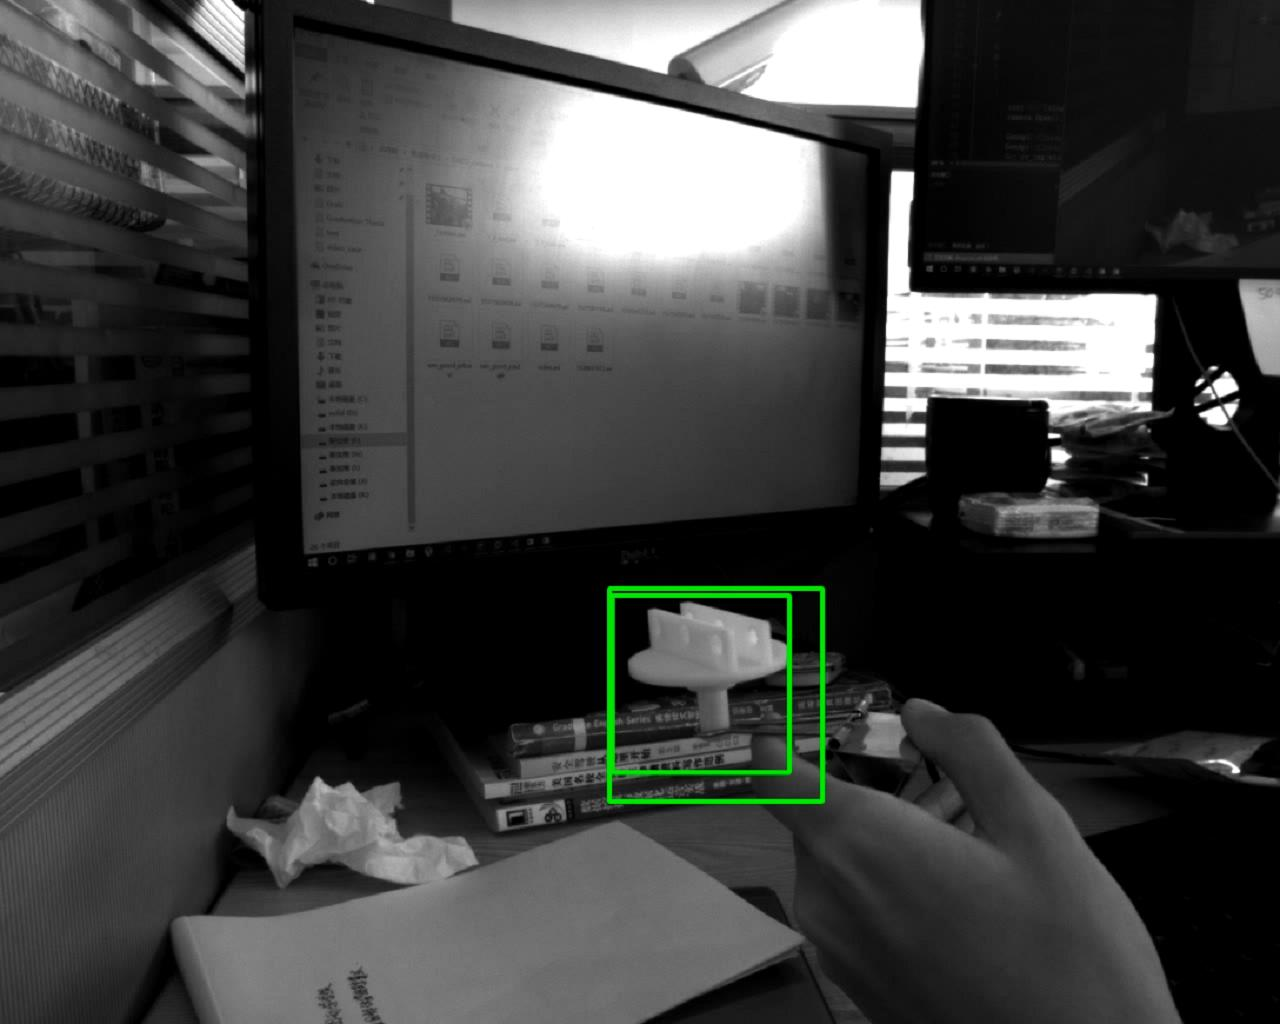
\includegraphics[height=3cm]{duojian1}\hspace{0.1em}
            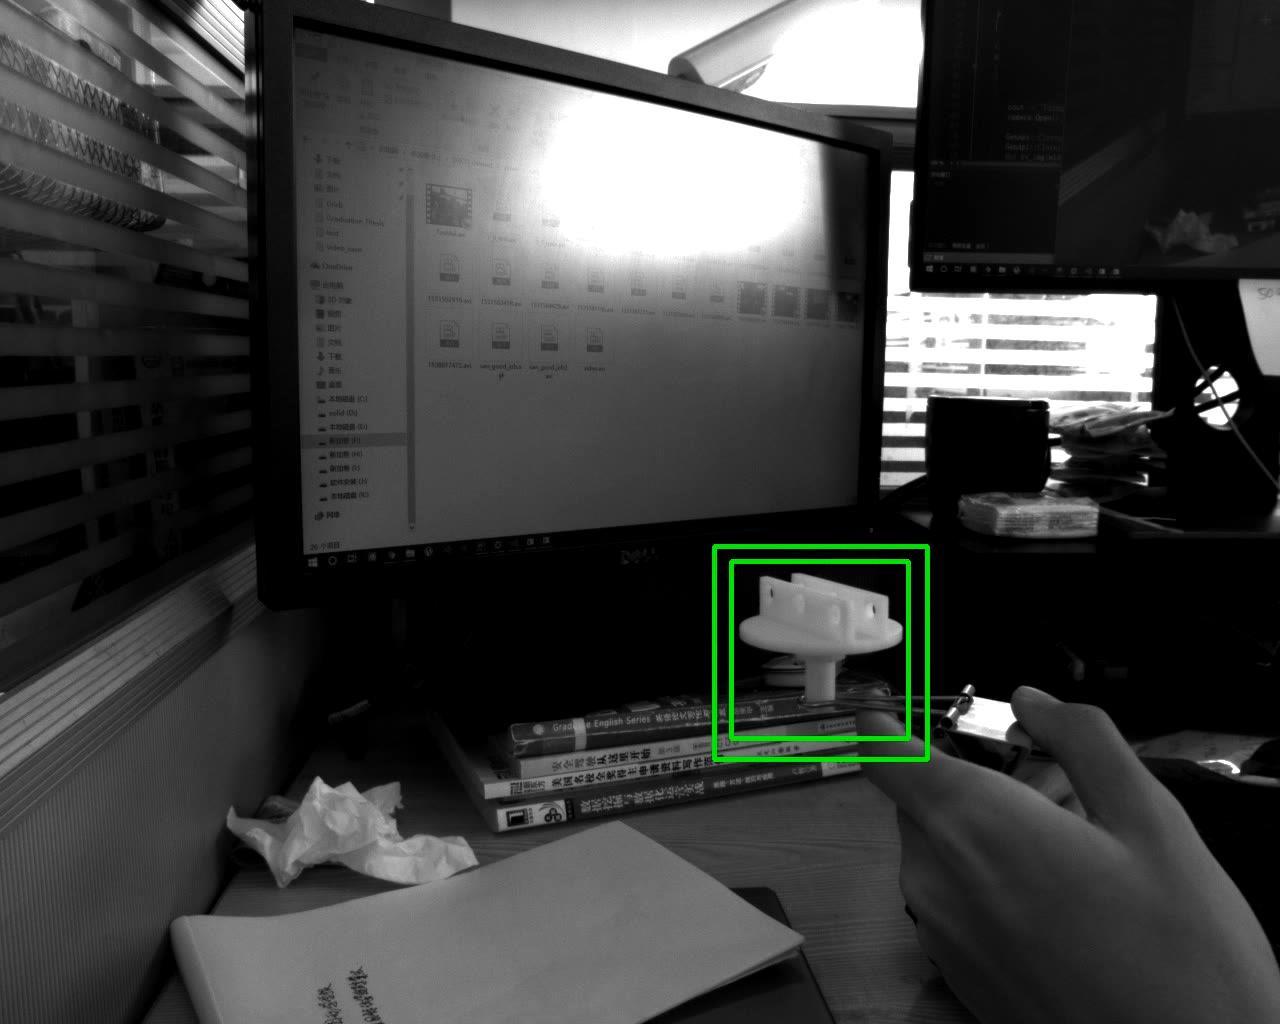
\includegraphics[height=3cm]{duojian2}}
            \vskip 0.3cm
            %\captionsetup{aboveskip=0pt}
            %\captionsetup{belowskip=0pt}
            %\captionof{subfigure}{多检}
            \subcaptionbox{误检\label{fig:chap05:err_detec}}{
            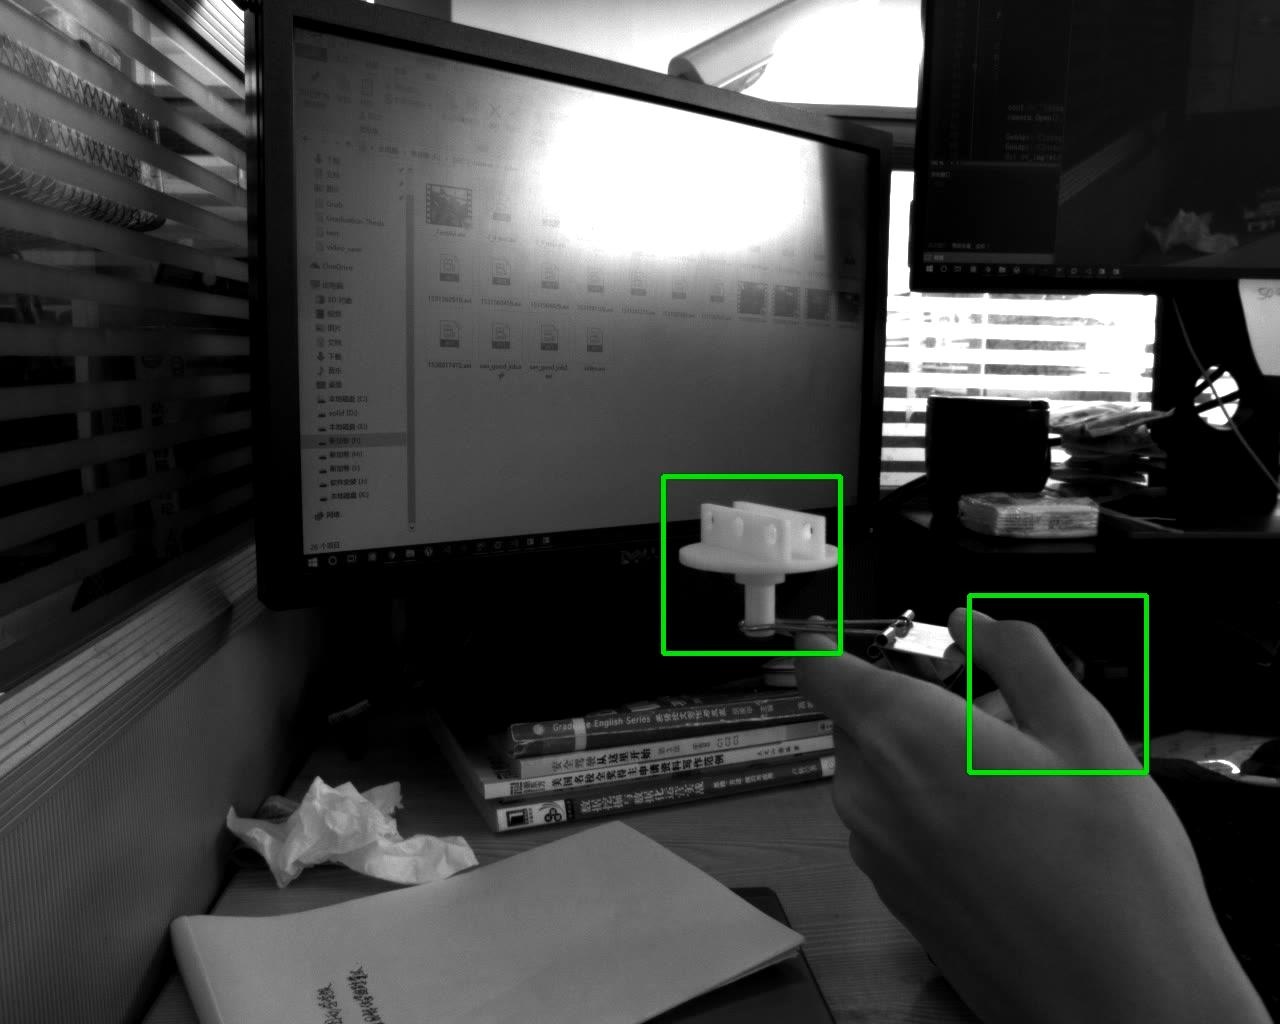
\includegraphics[height=3cm]{wujian1}\hspace{0.1em}
            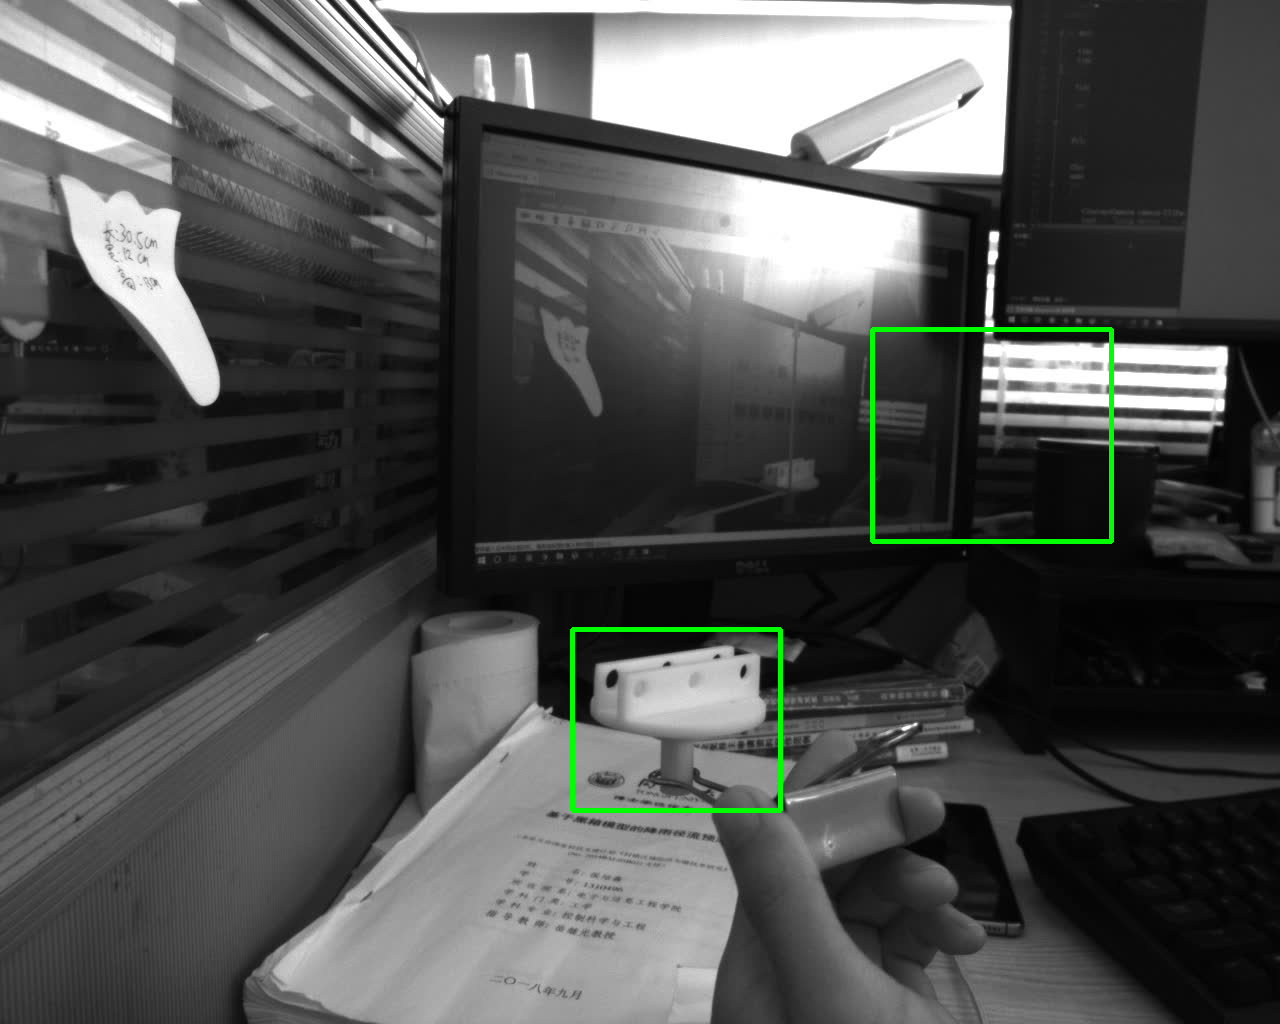
\includegraphics[height=3cm]{wujian2}}
            %\captionof{subfigure}{误检}\label{fig:chap05:err_detec}
            \captionof{figure}{多检、误检情况}
            \label{fig:chap05:double_detec_error_detec}
    \end{minipage}
    \hfill
    \begin{minipage}[c]{0.4\linewidth}
        \centering
        \captionof{table}{检测算法正检率}
         \label{table:chap05:detec_pos_test}
            \begin{tabular}{lcl}
                \toprule
                目标物体 & 姿态类别数 & 正检率(\%)   \\
                \midrule
                \multirow{3}*{圆盘固定件}    & \multirow{3}*{三分类} & 96.17\\ 
                ~    & ~ & 96.98 \\ 
                ~    & ~ & 94.78 \\ 
                \multirow{2}*{螺母}    & \multirow{2}*{两分类} & \color{blue}96.44\\ 
                ~    & ~ & \color{blue}94.35 \\ 
                \multirow{3}*{飞机模型}    & \multirow{3}*{三分类} & 94.18\\ 
                ~    & ~ & 95.17 \\ 
                ~    & ~ & 94.53 \\ 
                \multirow{2}*{五边形球体}    & \multirow{2}*{两分类} & \color{blue}96.64\\ 
                ~    & ~  & \color{blue}94.68 \\ 
                \bottomrule
            \end{tabular}
      \end{minipage}%
  \end{figure}



\begin{figure}[t] %[h]
    \centering% 
      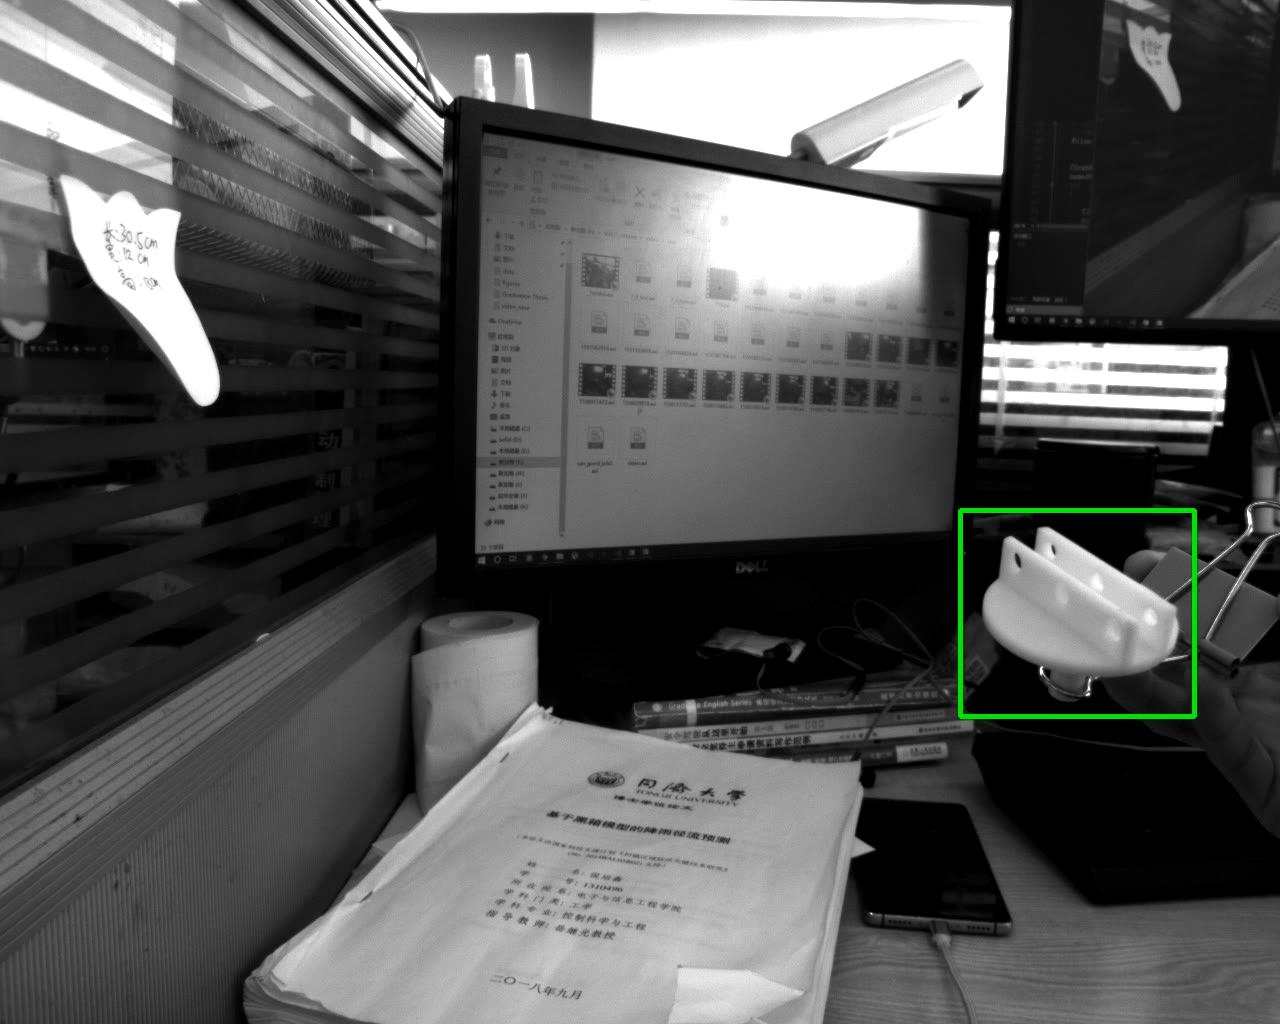
\includegraphics[height=3.8cm]{san_detc_1}
      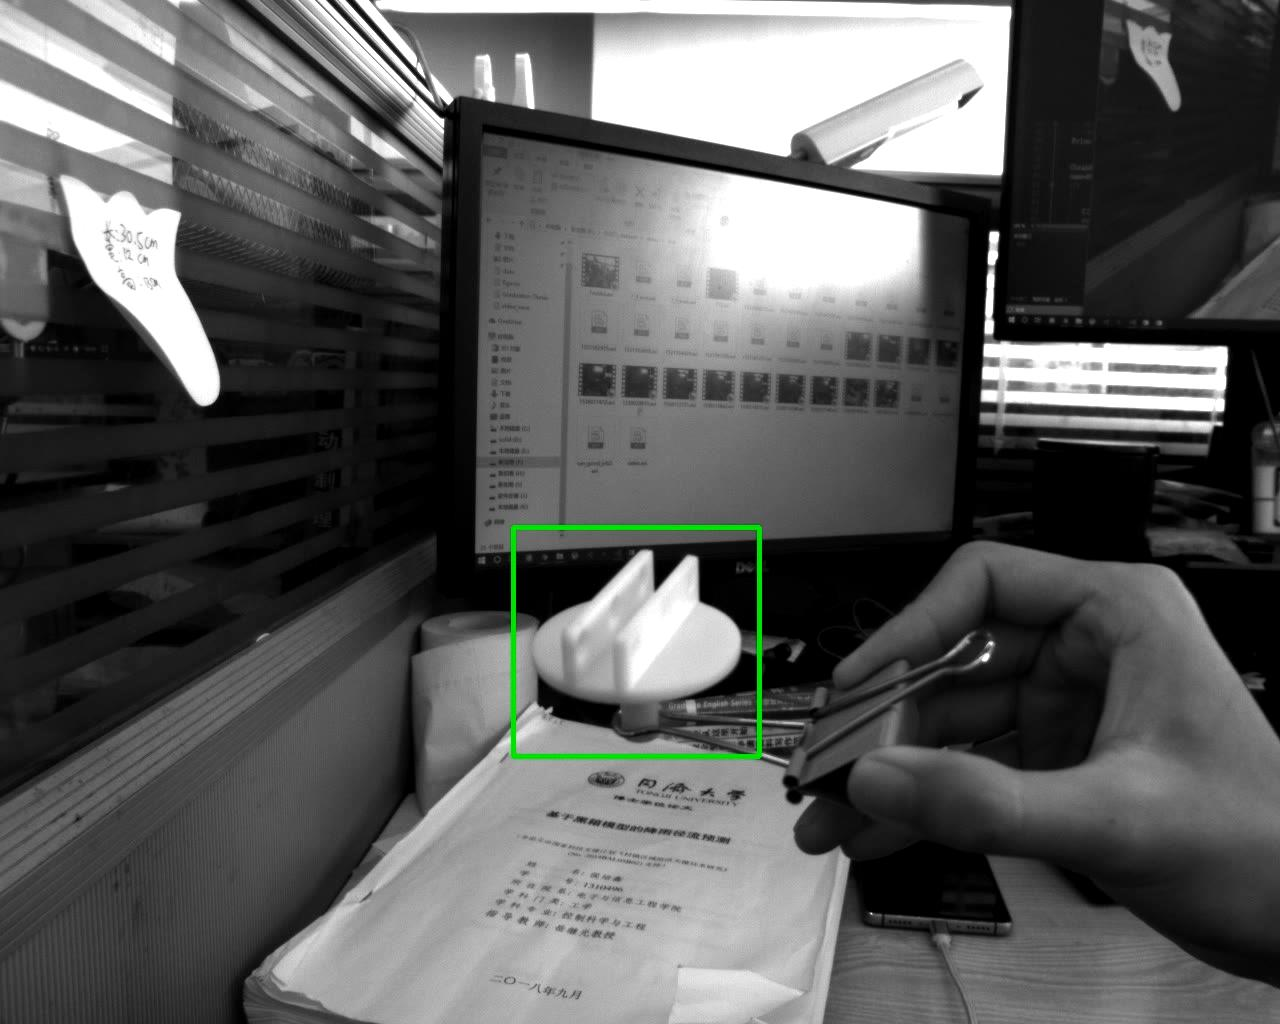
\includegraphics[height=3.8cm]{san_detc_2}
      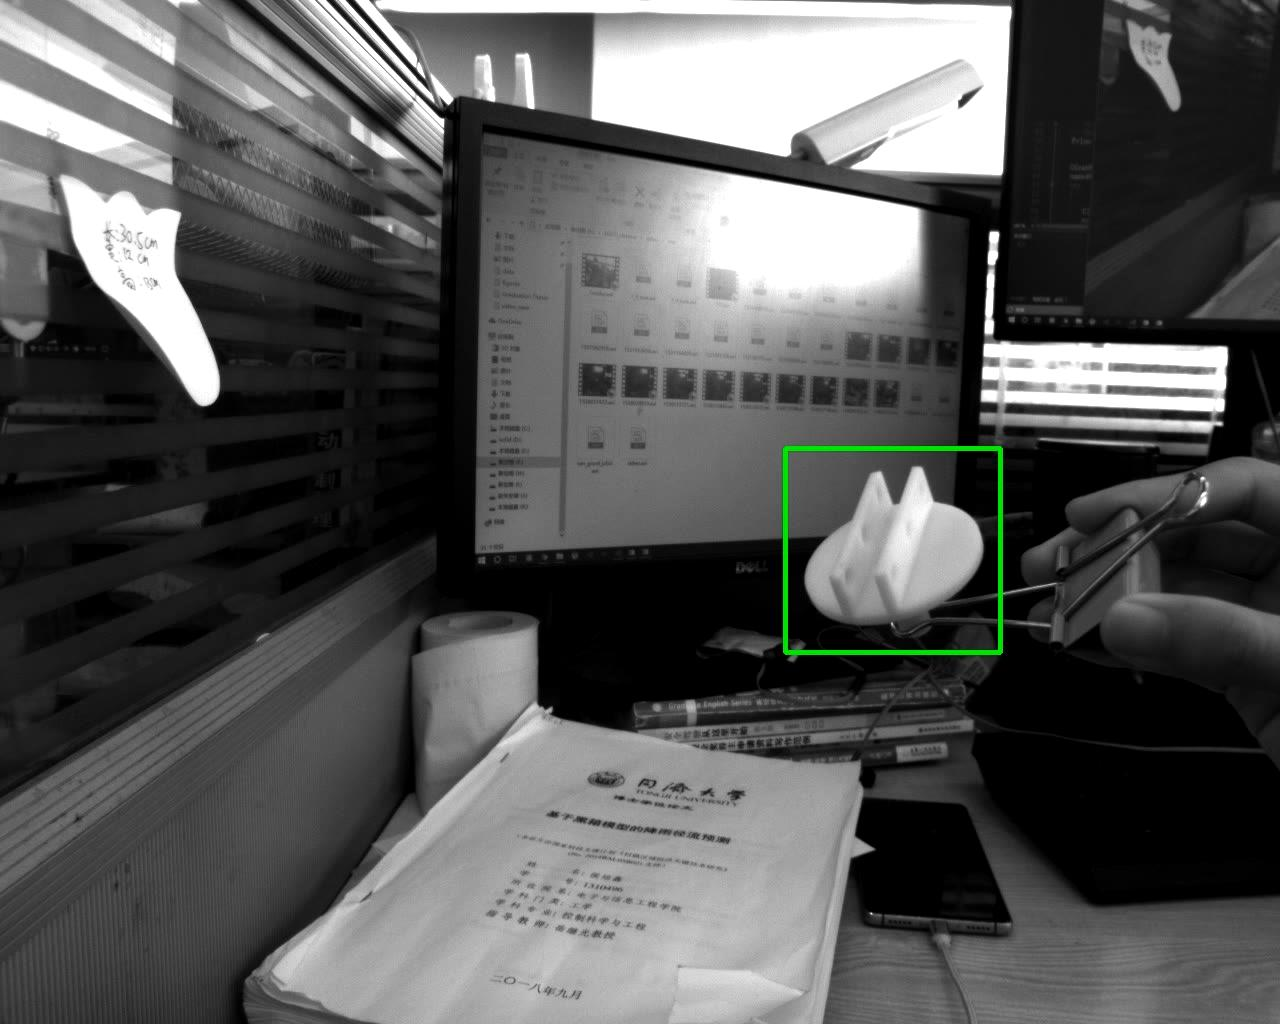
\includegraphics[height=3.8cm]{san_detc_3}
      \vskip 1pt
      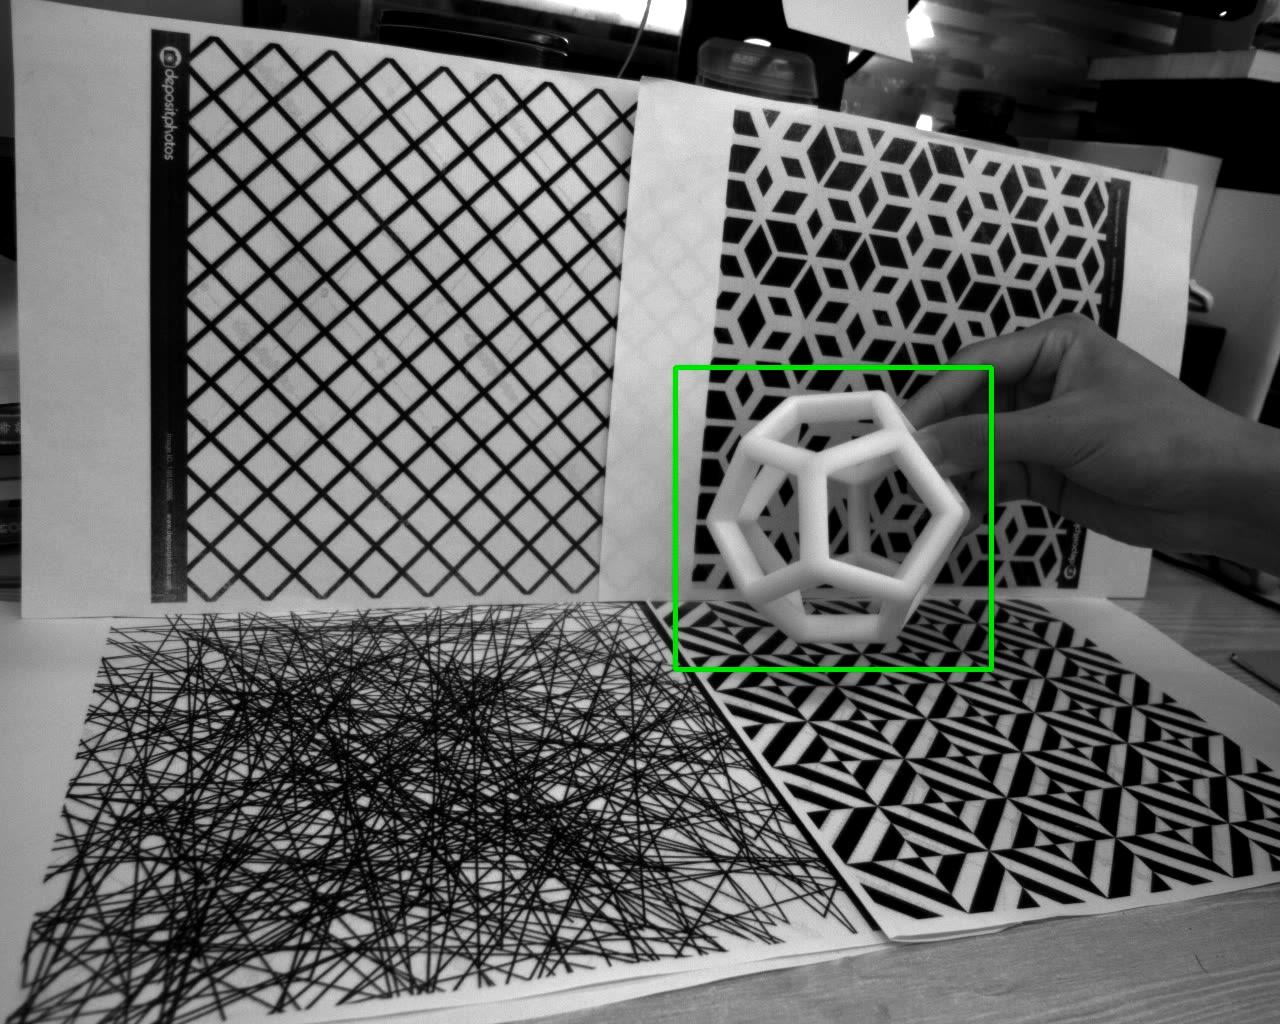
\includegraphics[height=3.8cm]{ball_detc_1}
      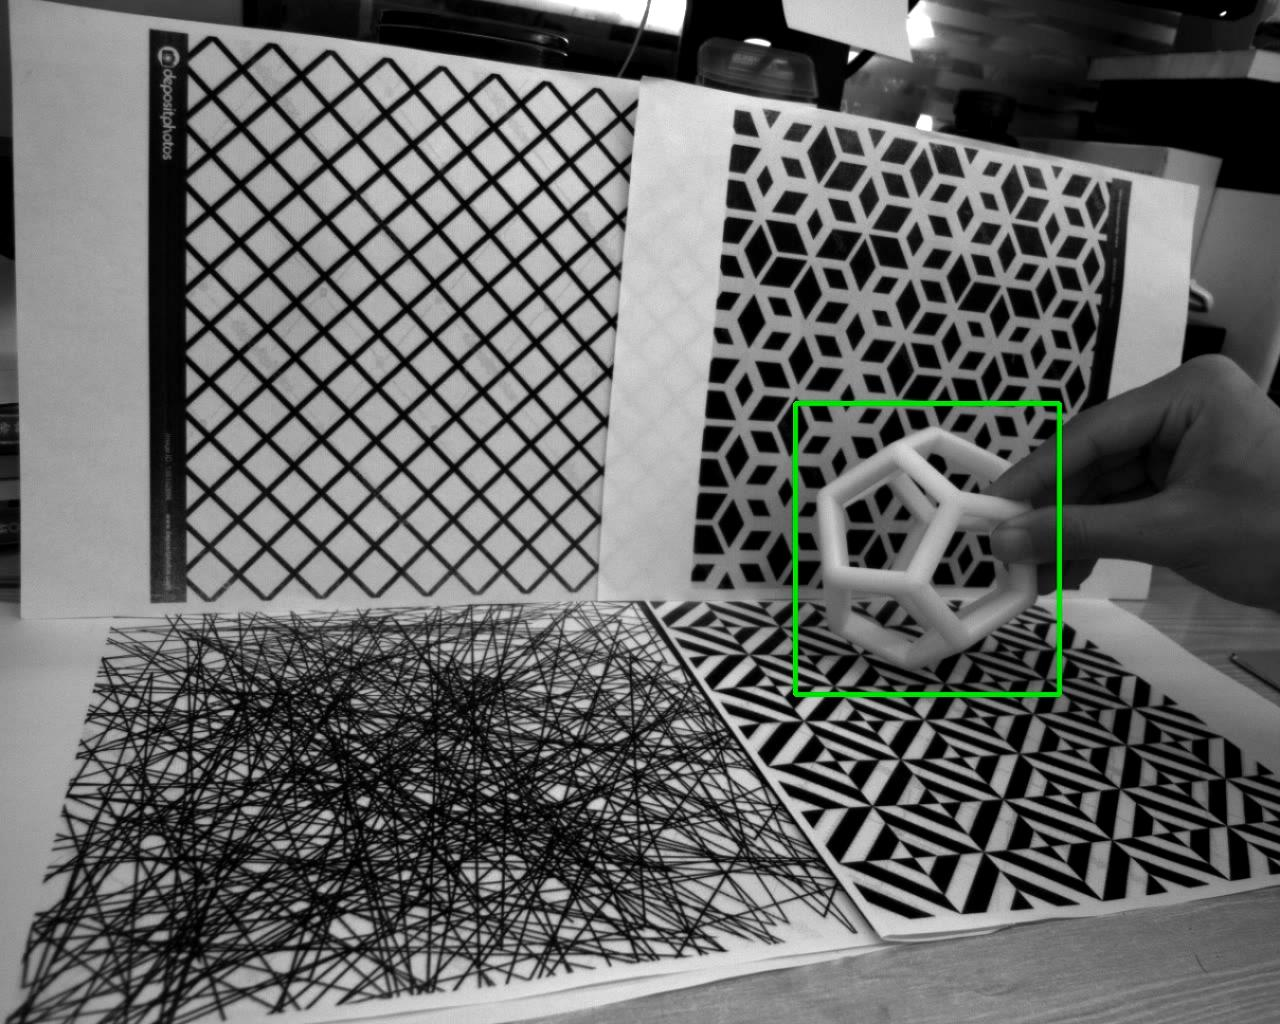
\includegraphics[height=3.8cm]{ball_detc_2}
      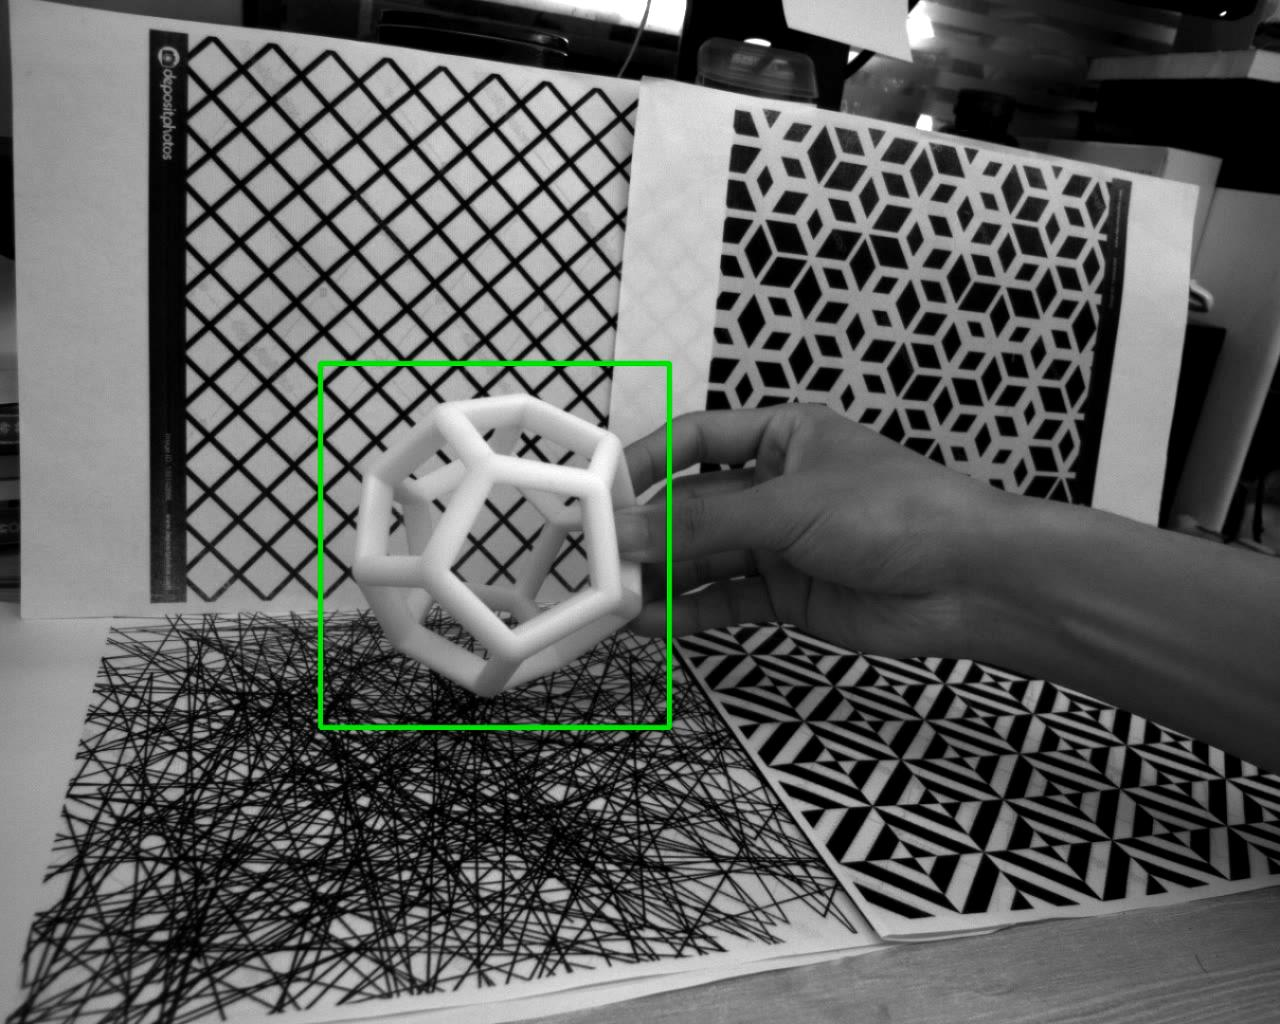
\includegraphics[height=3.8cm]{ball_detc_3}
      \vskip 1pt
      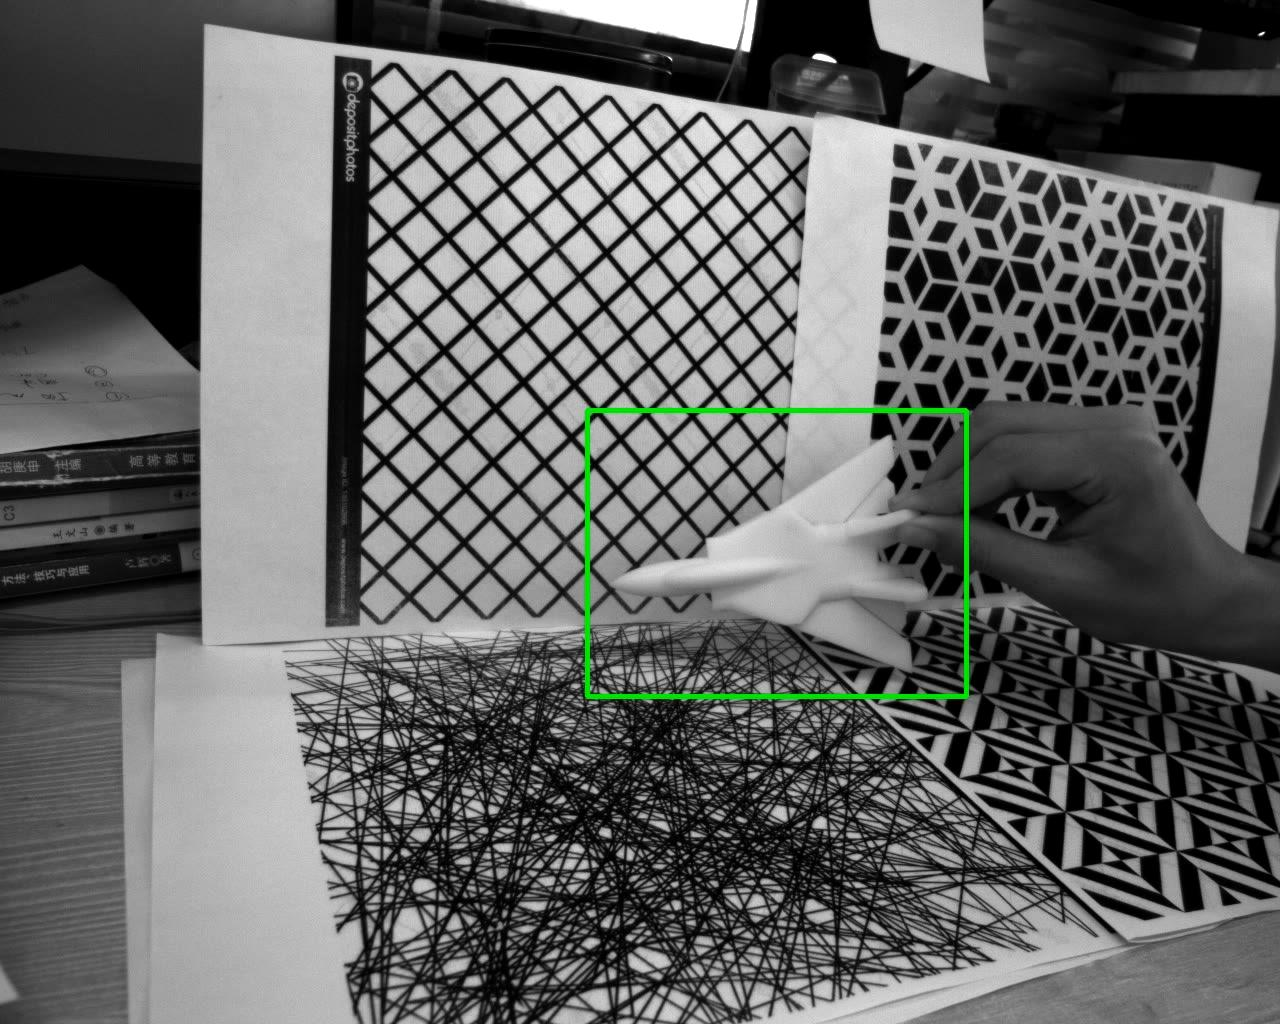
\includegraphics[height=3.8cm]{jet_detc_1}
      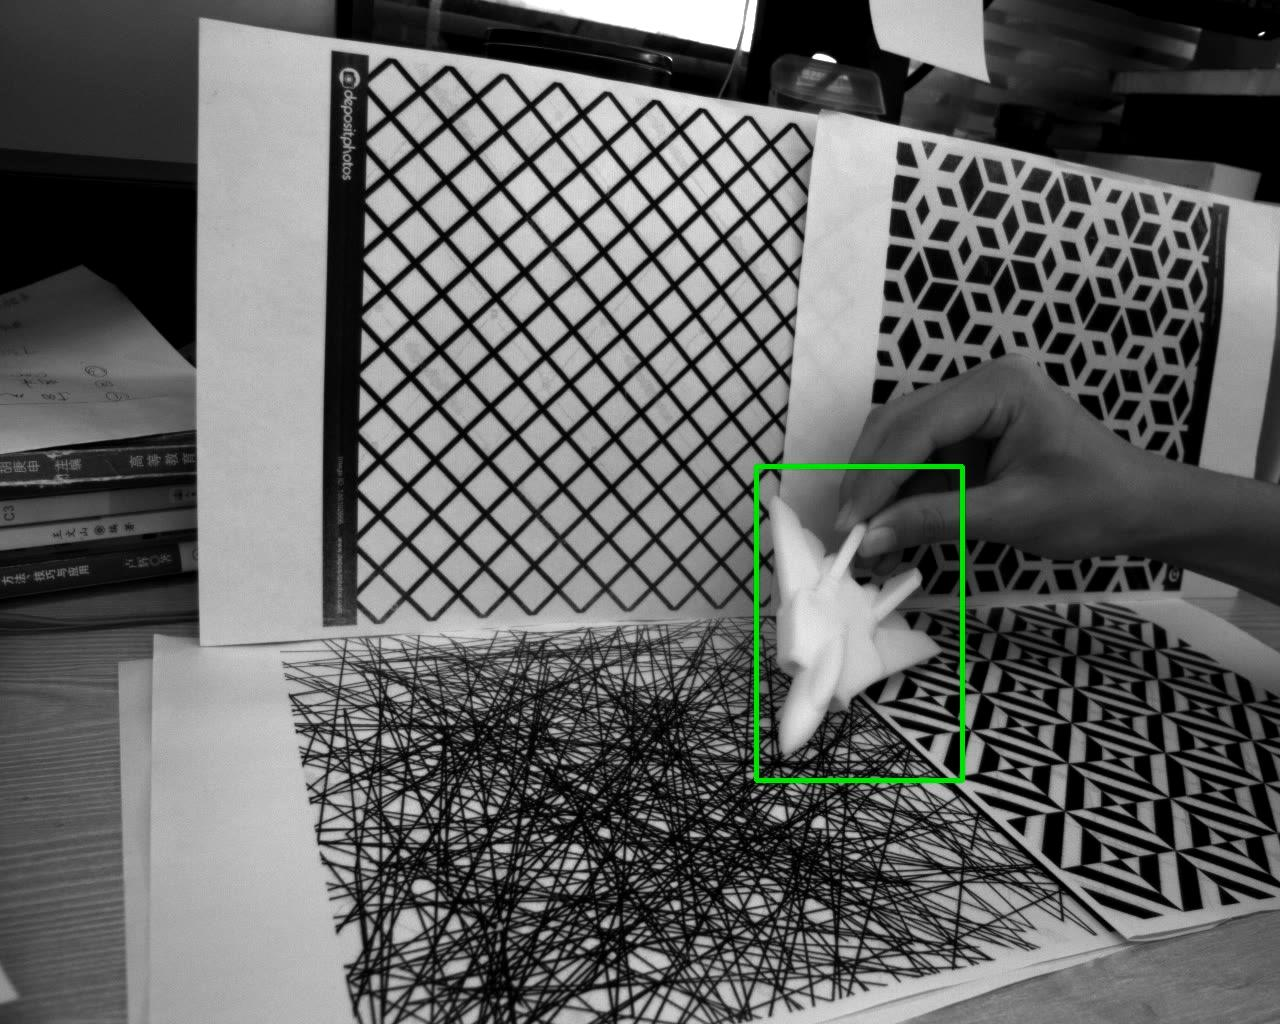
\includegraphics[height=3.8cm]{jet_detc_2}
      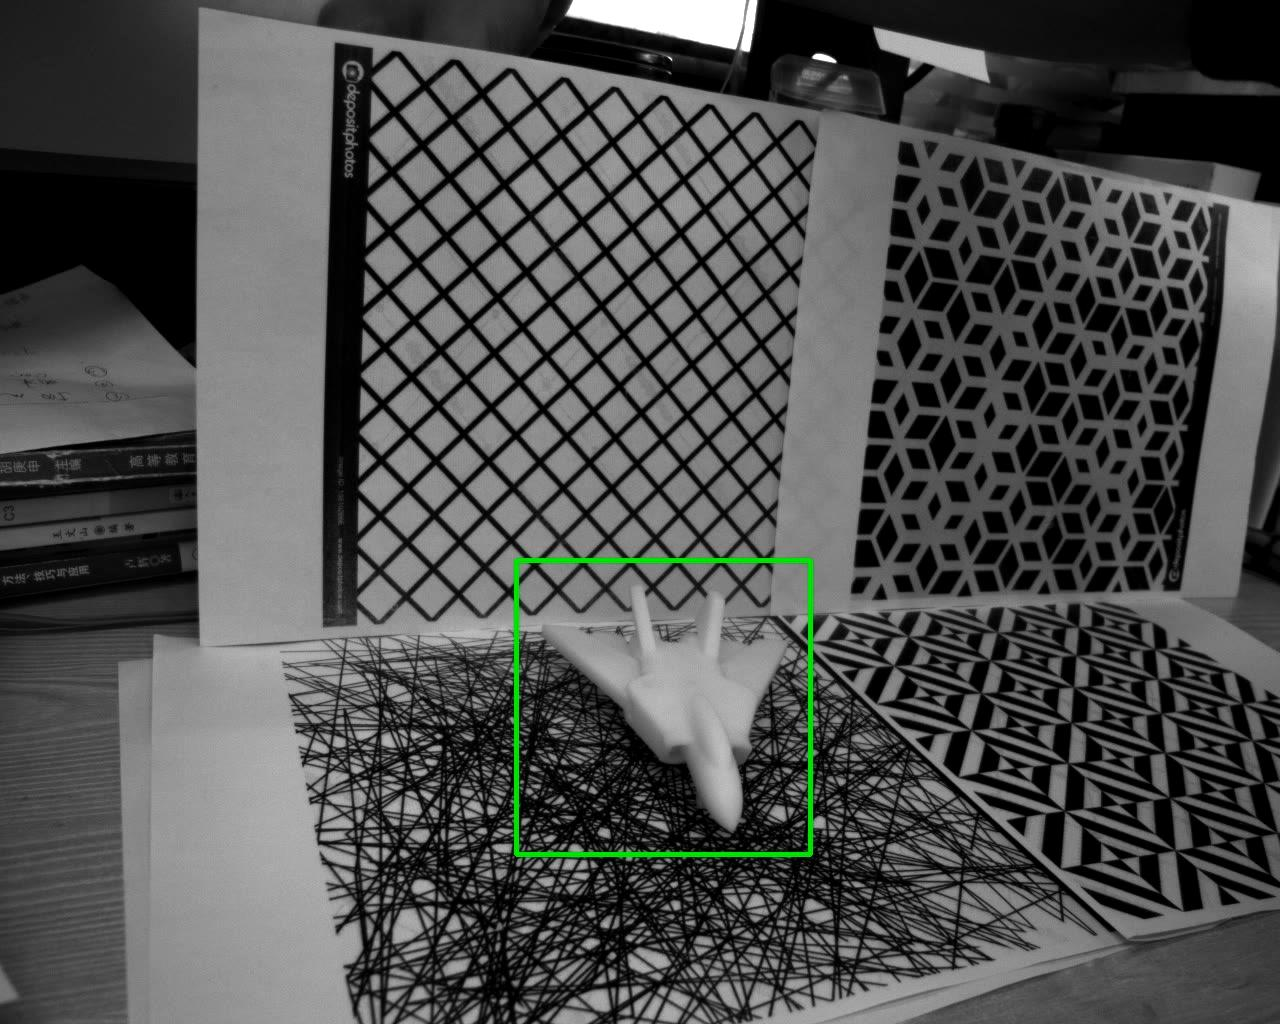
\includegraphics[height=3.8cm]{jet_detc_3}
      \vskip 1pt
      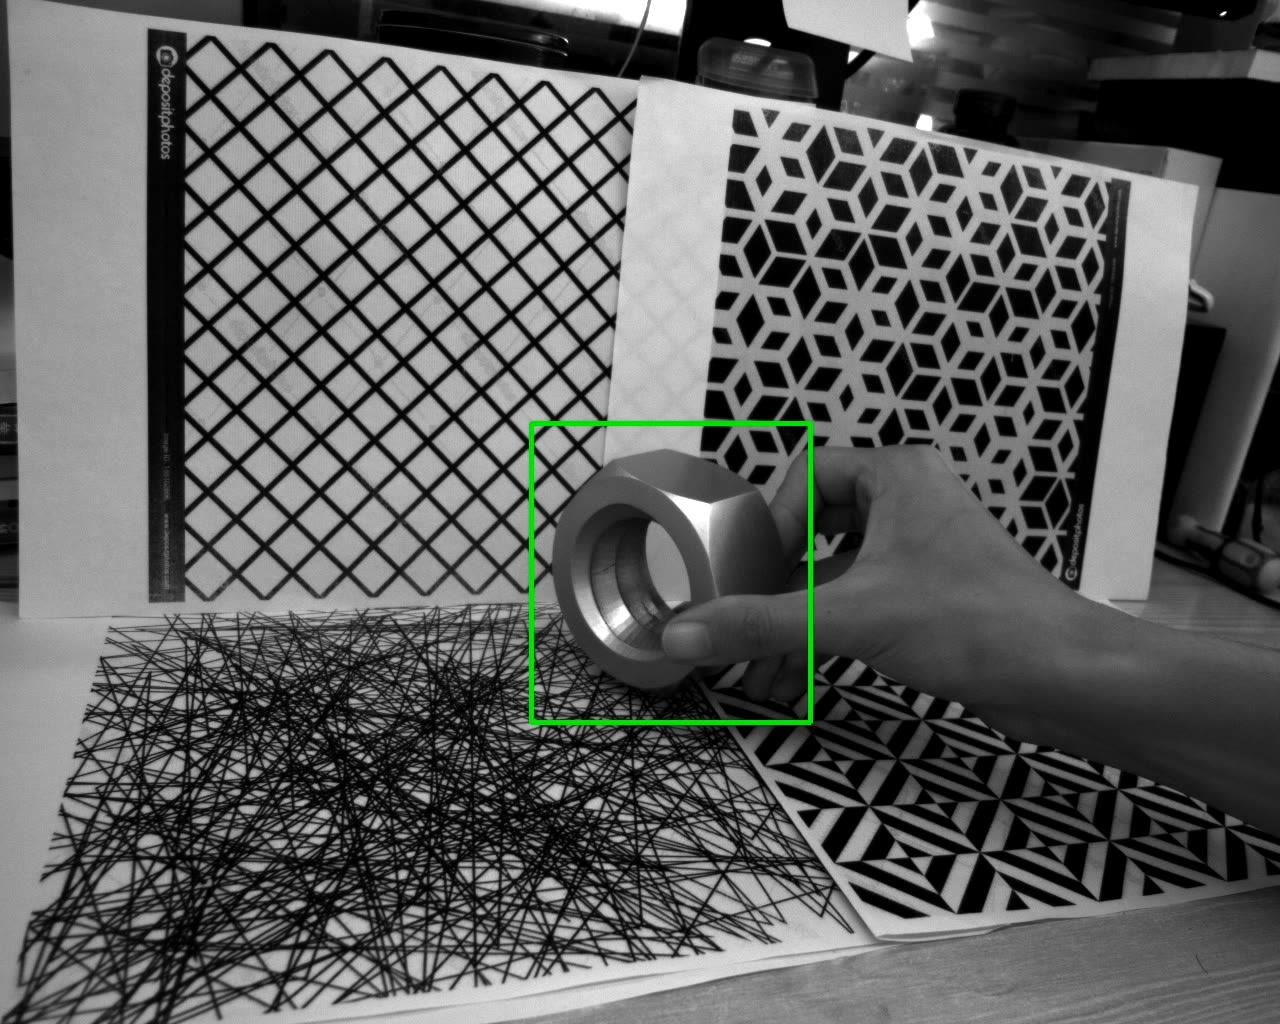
\includegraphics[height=3.8cm]{nut_detc_1}
      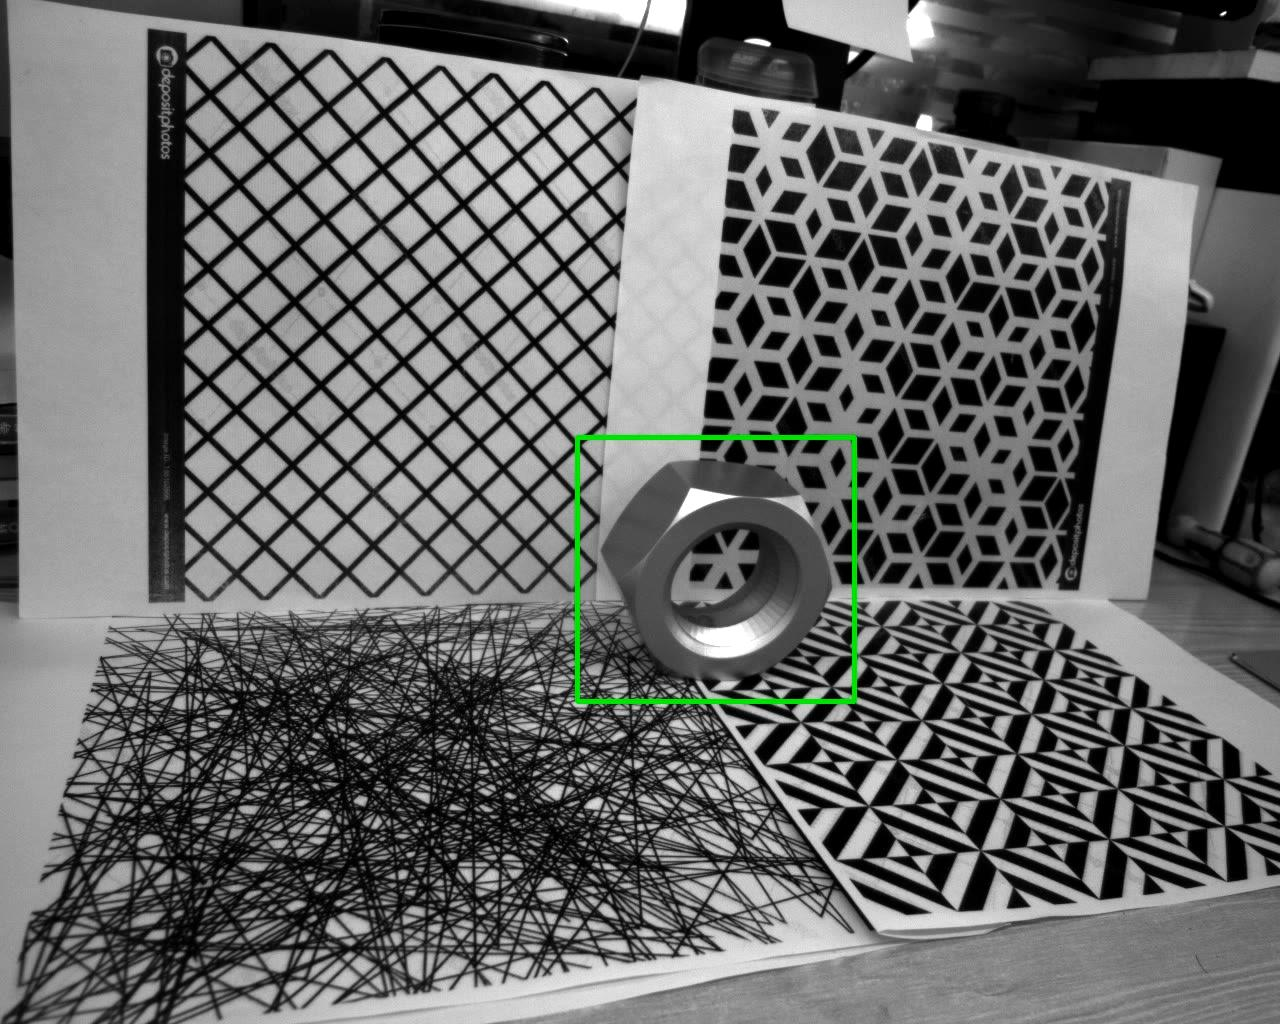
\includegraphics[height=3.8cm]{nut_detc_2}
      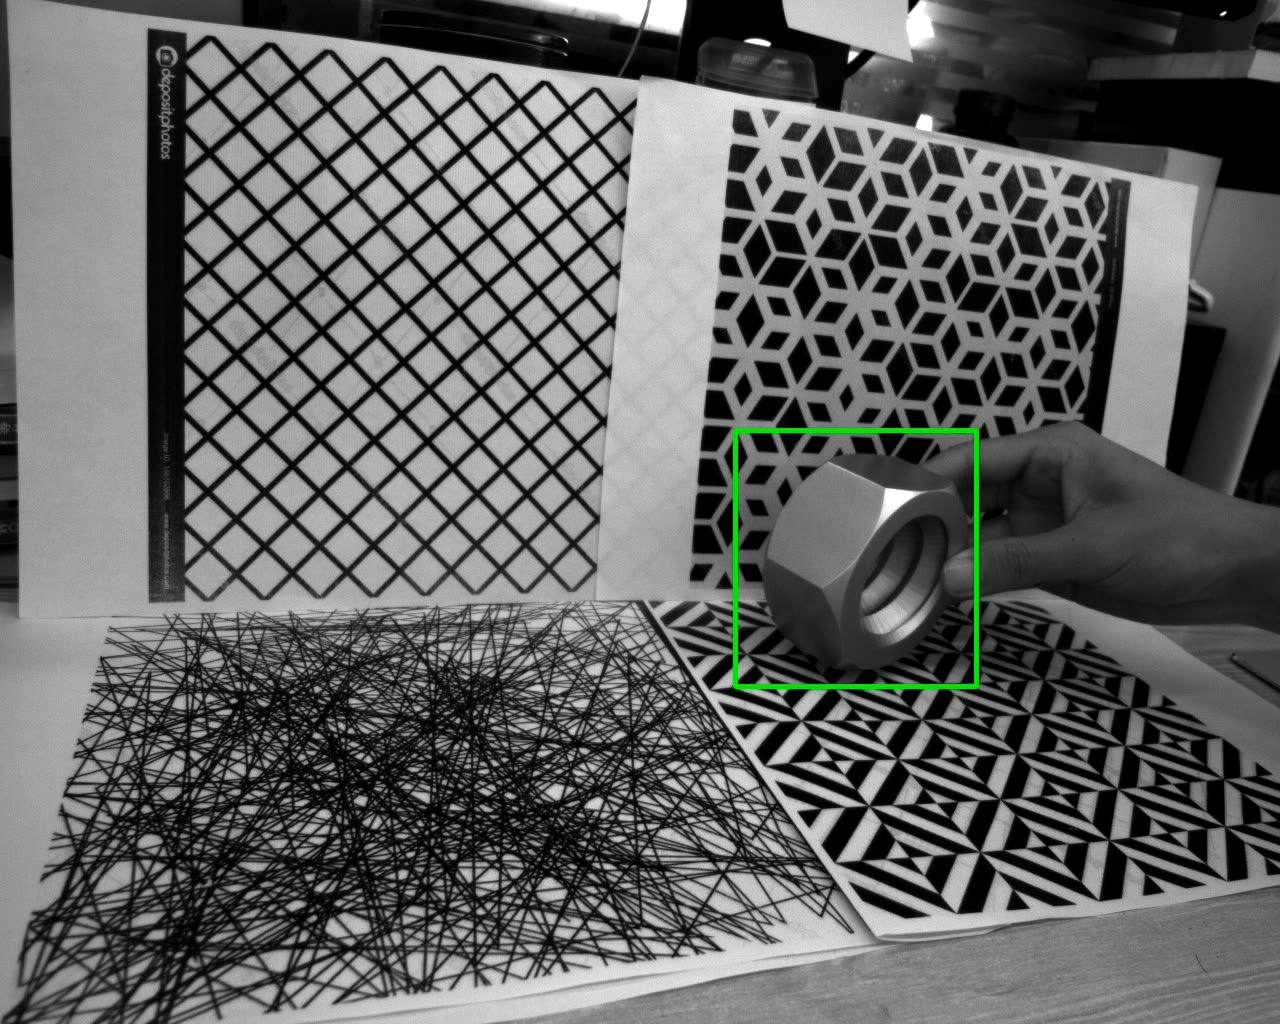
\includegraphics[height=3.8cm]{nut_detc_3}
    \caption{目标检测测试结果}
    \label{fig:chap05:obj_detec_test_res}
    \end{figure}


\subsection{平移向量回归测试}
\label{sec:trans_regress_test}
完成目标物体检测后,使用检测框的顶点坐标及尺寸信息作为特征,回归目标物体相对于相机的平移向量。本文针对所有目标物体单独训练了对应的回归模型,通过检测得到的分类结果选择相应的
模型进行平移向量回归。如图~\ref{fig:chap05:video_trans_regre}~所示为使用检测算法对测试视频的每一帧图像进行物体检测,之后将结果作为回归模型的输入,以得到算法对平移向量的估计。该视频是以圆盘固定件作为测试物体,
图中的蓝色曲线为回归的结果,橙色曲线为平移向量的真值,根据统计计算~x~轴的向量估计平均误差为~$0.92$~毫米,~y~轴平均误差为~$0.79$~毫米,
~z~轴平均误差为~$-2.72$~毫米。z~轴估计误差高于其余两轴,该轴方向是由相机光心出发,垂直于成像平面的,其值代表物体中心相对于相机的深度,在使用单目相机对深度进行估计时,主要通过检测到的物体大小及其模型信息以得到其深度。
在本文中利用检测框的大小代表物体的大小进行回归,然而使用滑窗的方法会导致检测框的不稳定,出现如图~\ref{fig:chap05:double_detc}~所示的多检情况,由此导致回归算法的抖动以及误差。因此在~z~轴上的深度检测误差是由于上级
检测算法导致的误差,该误差将在模板匹配中进行消除。表~\ref{table:chap05:regre_dataset}~所示为所有物体的平移向量回归误差,表中对物体的所有粗分类位姿进行了整合统计。通过比较可知,当物体所占的图像区域,也即检测框的大小
越大时,估计的平移向量越准确,分析原因应该是数据库的遍历问题,检测框越大,遍历完所有图像位置所需的图片数量也就越少,模型的在图像区域中可能出现的平移向量数量也就越少,也即对于不同的目标物体,准备了相同数量的
训练样本,但检测框越大的物体对应的样本空间越小,所以估计的精度越高,而小物体由于样本空间较大,可能的取值更多,导致精度相比较低。

\begin{figure}[t] %[h]
    \centering% 
    \subcaptionbox{x轴平移\label{fig:chap05:regre_x}}{
      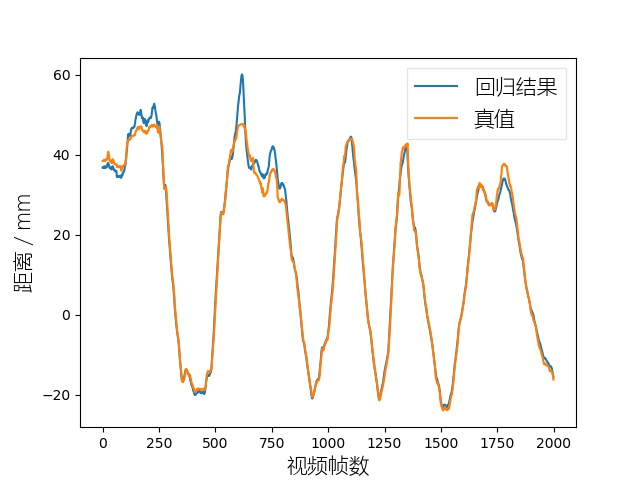
\includegraphics[height=3.5cm]{regre_trans_x}}
    \subcaptionbox{y轴平移\label{fig:chap05:regre_y}}{
      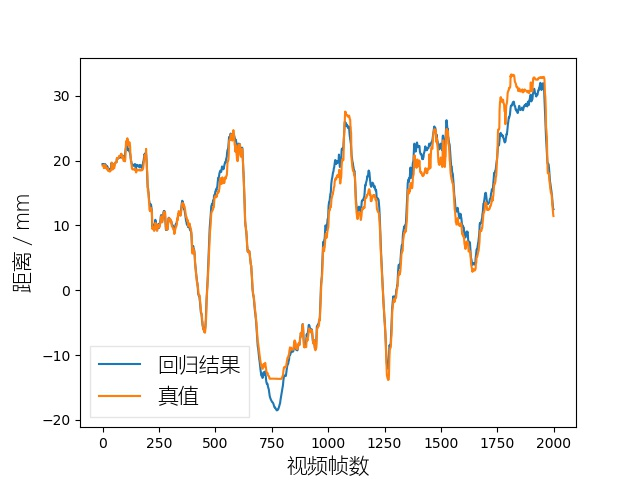
\includegraphics[height=3.5cm]{regre_trans_y}}
    \subcaptionbox{z轴平移\label{fig:chap05:regre_z}}{
      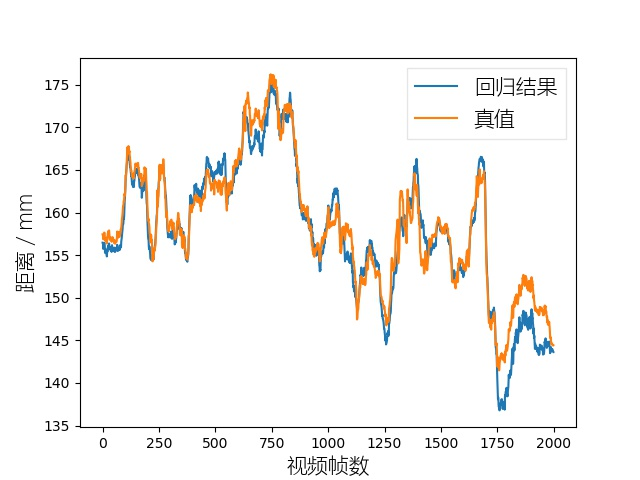
\includegraphics[height=3.5cm]{regre_trans_z}}
    \caption{平移向量回归模型测试}
    \label{fig:chap05:video_trans_regre}
    \end{figure}

\begin{table}[t]
    \centering
    \caption{平移向量回归的平均误差}
    \label{table:chap05:regre_dataset}
    \begin{tabular}{lccc}
        \toprule
        目标物体 &  x~轴误差(~$mm$~)   &y~轴误差(~$mm$~)   & z~轴误差(~$mm$~)   \\
        \midrule
        圆盘固定件   & 0.92 & 0.79 & -2.72\\ 
        螺母  & 0.86 & 0.70 & -1.25 \\ 
        飞机模型  & 0.74 & 0.39 & 1.46 \\ 
        五边形球体  & 0.82 & 0.47 & -1.75\\ 
        \bottomrule
    \end{tabular}
    \end{table}


\subsection{模板匹配测试}
\label{sec:template_test}
测试模板匹配的效果,主要考虑出现误检以及多检时能否正确判断,以得到准确的初始化位姿。

\noindent{\textbf{误检}}

发生误检时,模板匹配将得到多个平移向量的输入,其中包含正确的平移向量,也包含错误的平移向量。根据给出的平移向量以及对应的粗分类模板,将物体模型的光栅点映射到图像平面。之后利用所有模板构建的位姿,
运行模型与边缘图像的匹配算法,得到匹配后的位姿,根据该位姿判断模型匹配的权重,如图~\ref{fig:chap05:error_pose_match}~所示,由于背景干扰导致检测算法在物体右上侧出现误检,在将模型光栅点移动到误检区域并运行
匹配算法后,得到的边缘光栅点权重明显低于正检区域,因此初始化算法将以正检区域的结果作为输出,位姿结果如图中的三轴坐标系所示。

\noindent{\textbf{多检}}

发生多检时,模板匹配模块将得到多个比较接近的平移向量,本文将按序遍历该平移向量,通过模板构建相应的位姿,并运行匹配算法。当匹配的权重大于一定阈值后就退出循环,不再遍历后续的位姿,如图~\ref{fig:chap05:multi_pose_match}~所示。
本文试验通过遍历所有的位姿,以寻找最优的匹配权重对应的位姿作为初始化位姿输出,但结果中存在多个权重很高且数值十分相近的位姿,使用其中任意一个作为初始化位姿都能实现追踪算法的初始化,并且遍历所有位姿的方法运行
耗时较长,由此在发生多检时,仅寻找第一个能够高于预设定阈值的位姿作为初始化位姿输出,算法在初始化的成功率以及时效性上都能获得比较理想的效果。

根据检测结果选择不同的粗分类姿态模板库,以寻找输入图片中目标物体的初始化位姿。设定位姿匹配的阈值,在完成配准后计算光栅点匹配的得分,当配准得分高于设定阈值时,结束寻找过程,
将该位姿作为初始化位姿进行输出。结果如图~\ref{fig:chap05:pose_estimate_template_match}~所示。通过测试,模板匹配的方法能够在检测出现一定误差的情况下配准目标物体,得到目标相对于相机坐标系的位姿,实现对追踪算法的
自动初始化。


\begin{figure}[t] %[h]
    \centering% 
    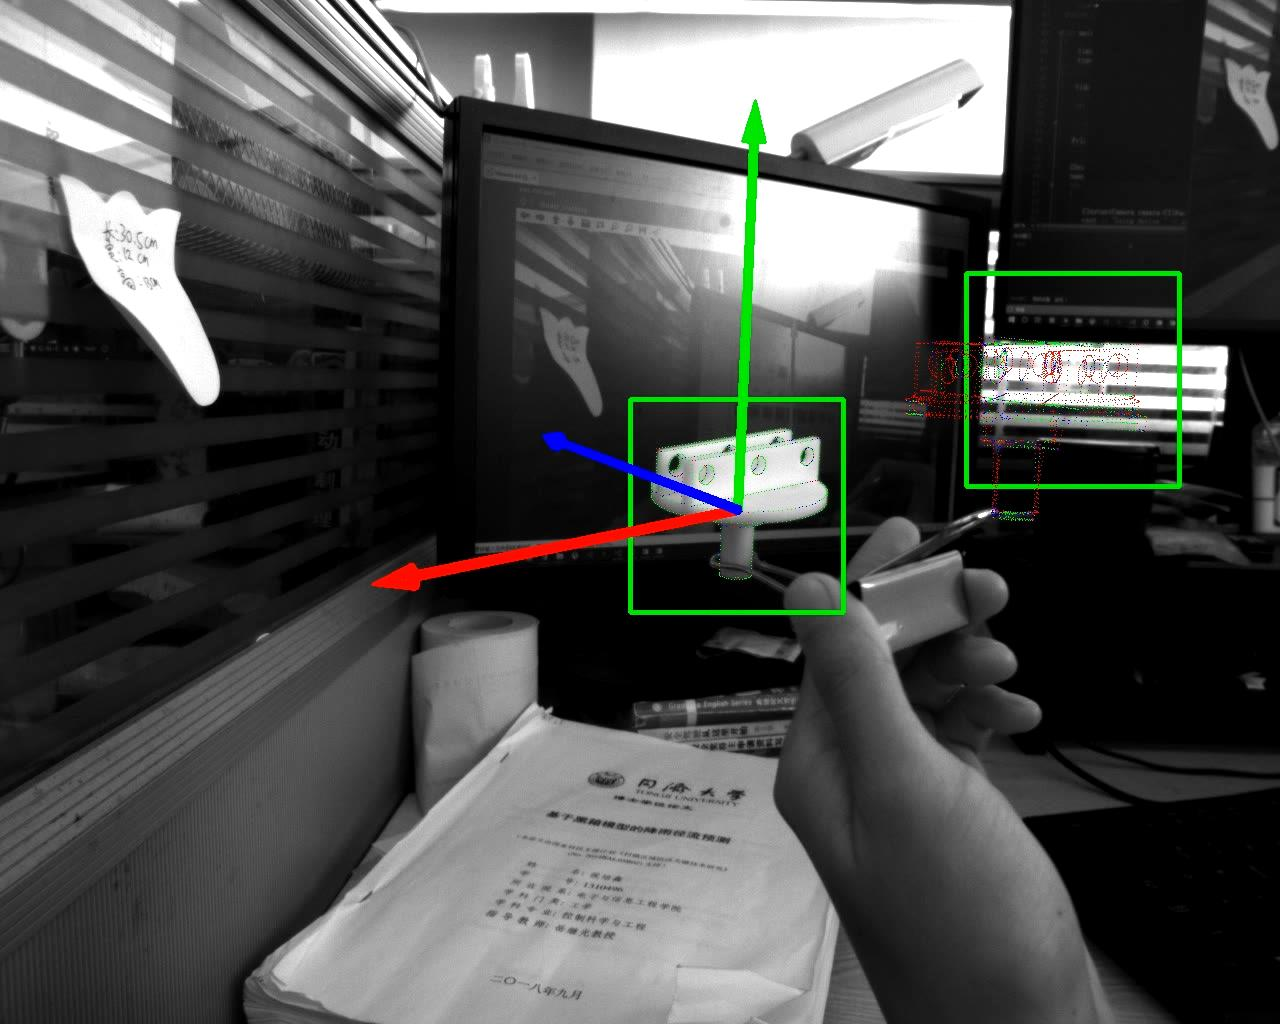
\includegraphics[height=3.8cm]{error_match_1}
    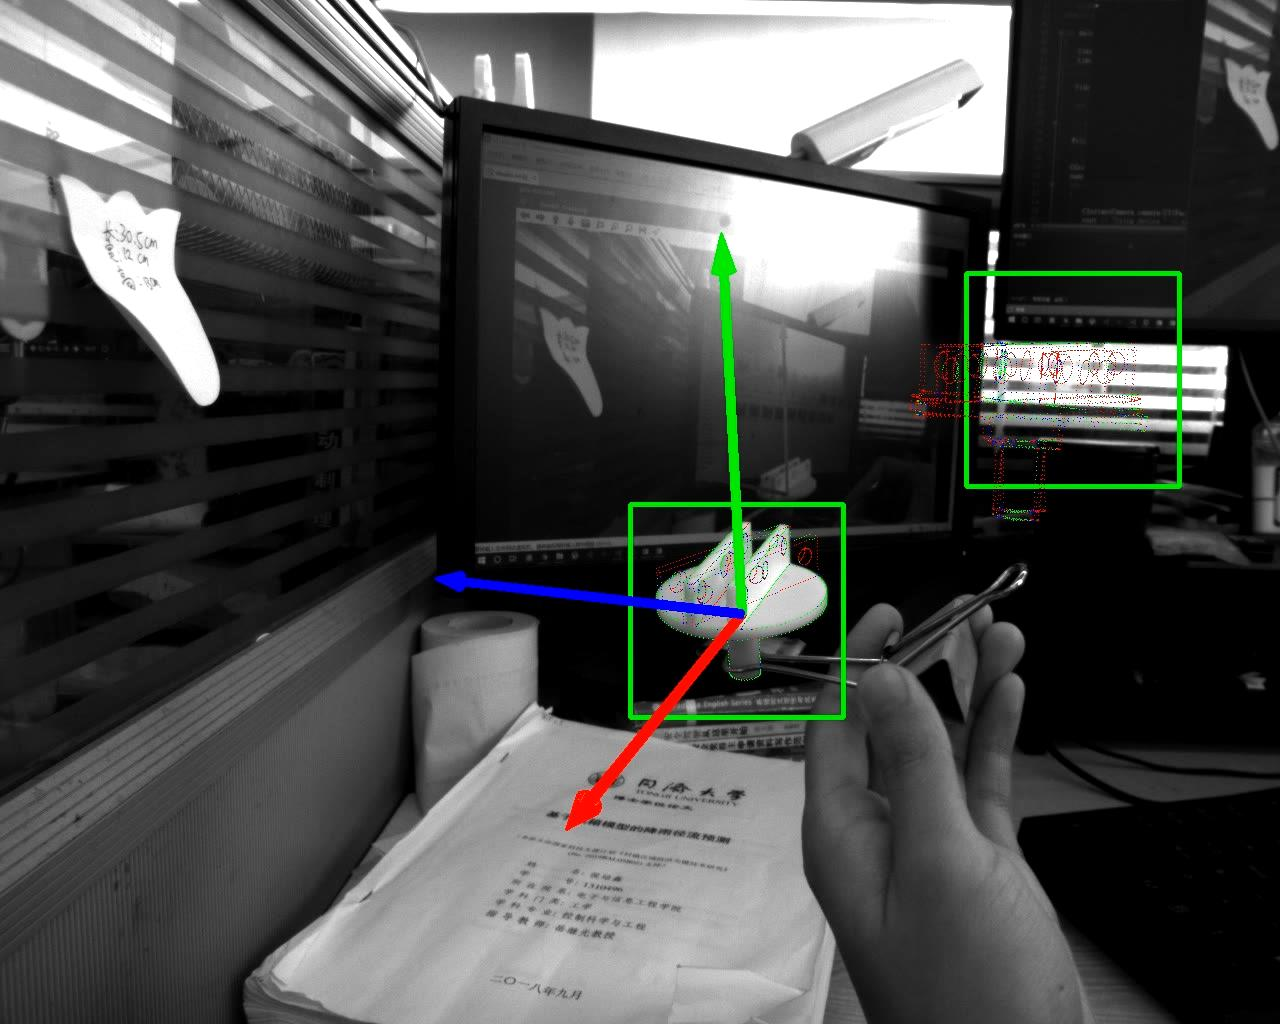
\includegraphics[height=3.8cm]{error_match_2}
    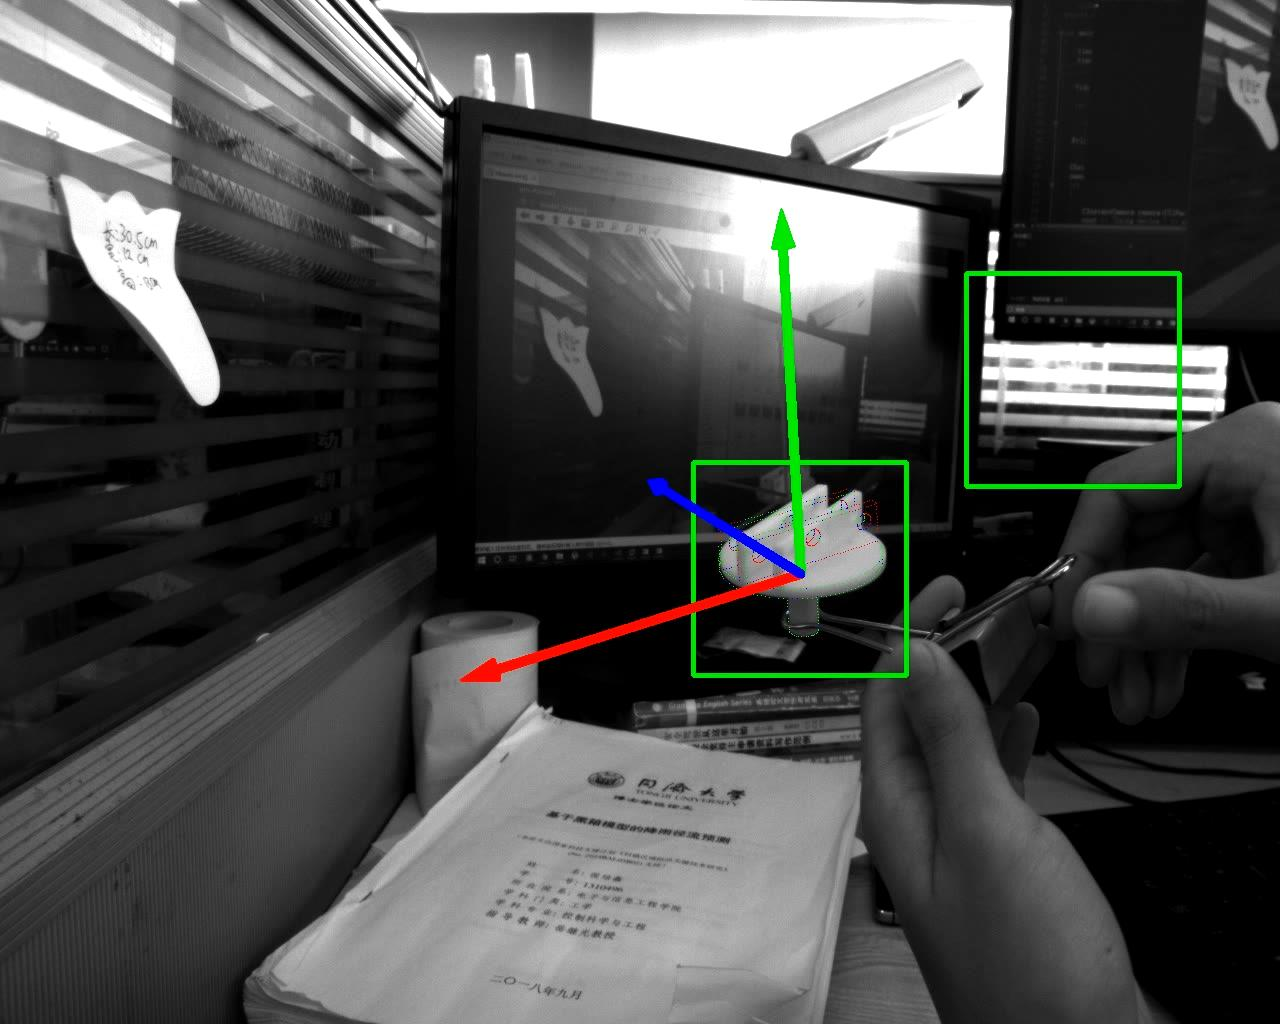
\includegraphics[height=3.8cm]{error_match_3}
    \caption{误检情况的模板匹配结果}
    \label{fig:chap05:error_pose_match}
    \end{figure}
\begin{figure}[t] %[h]
    \centering% 
    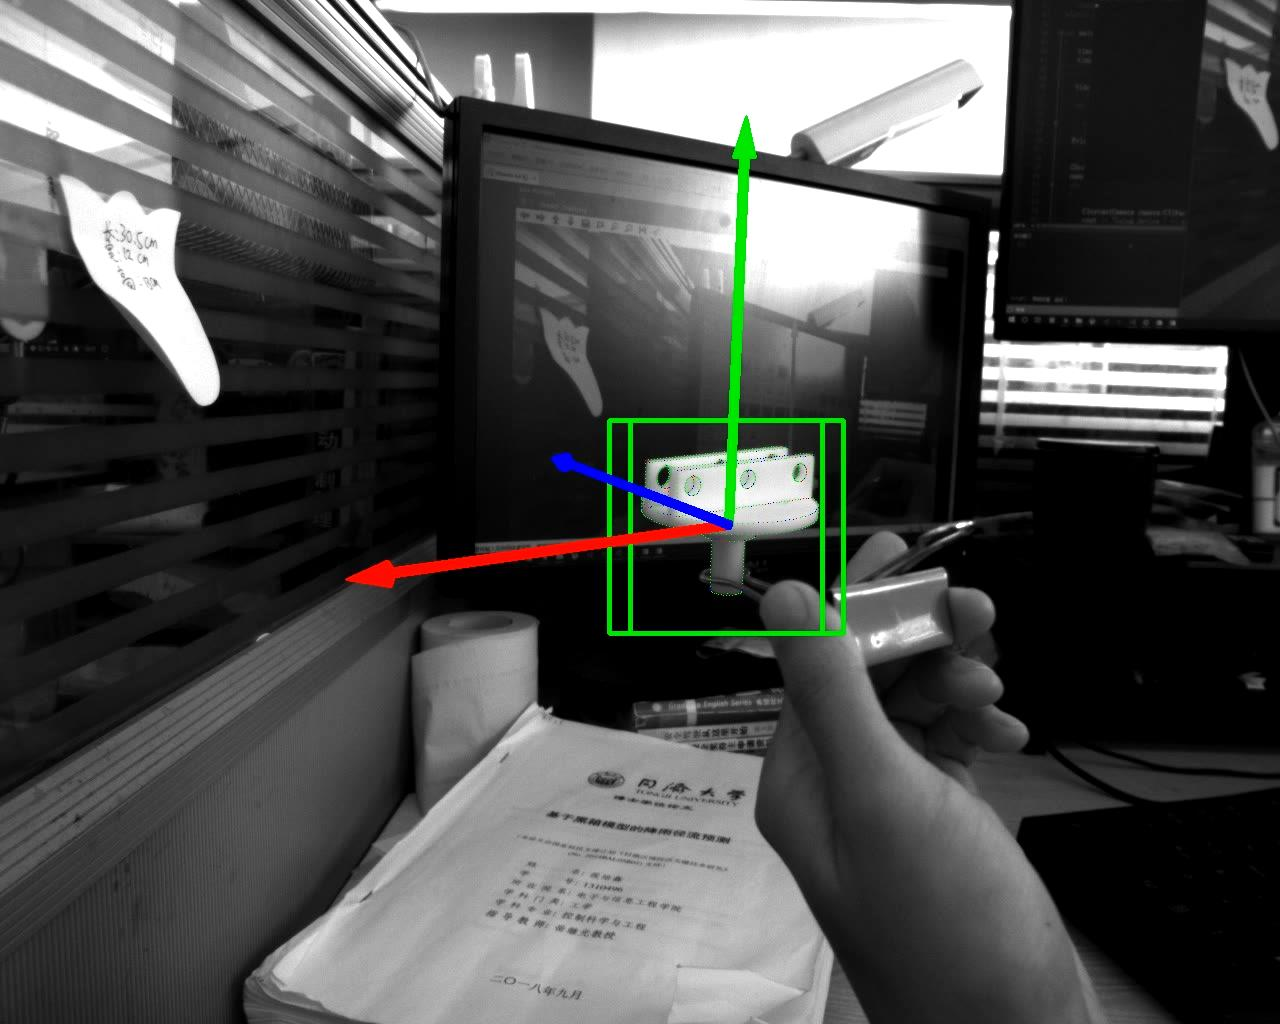
\includegraphics[height=3.8cm]{double_detec_pose1}
    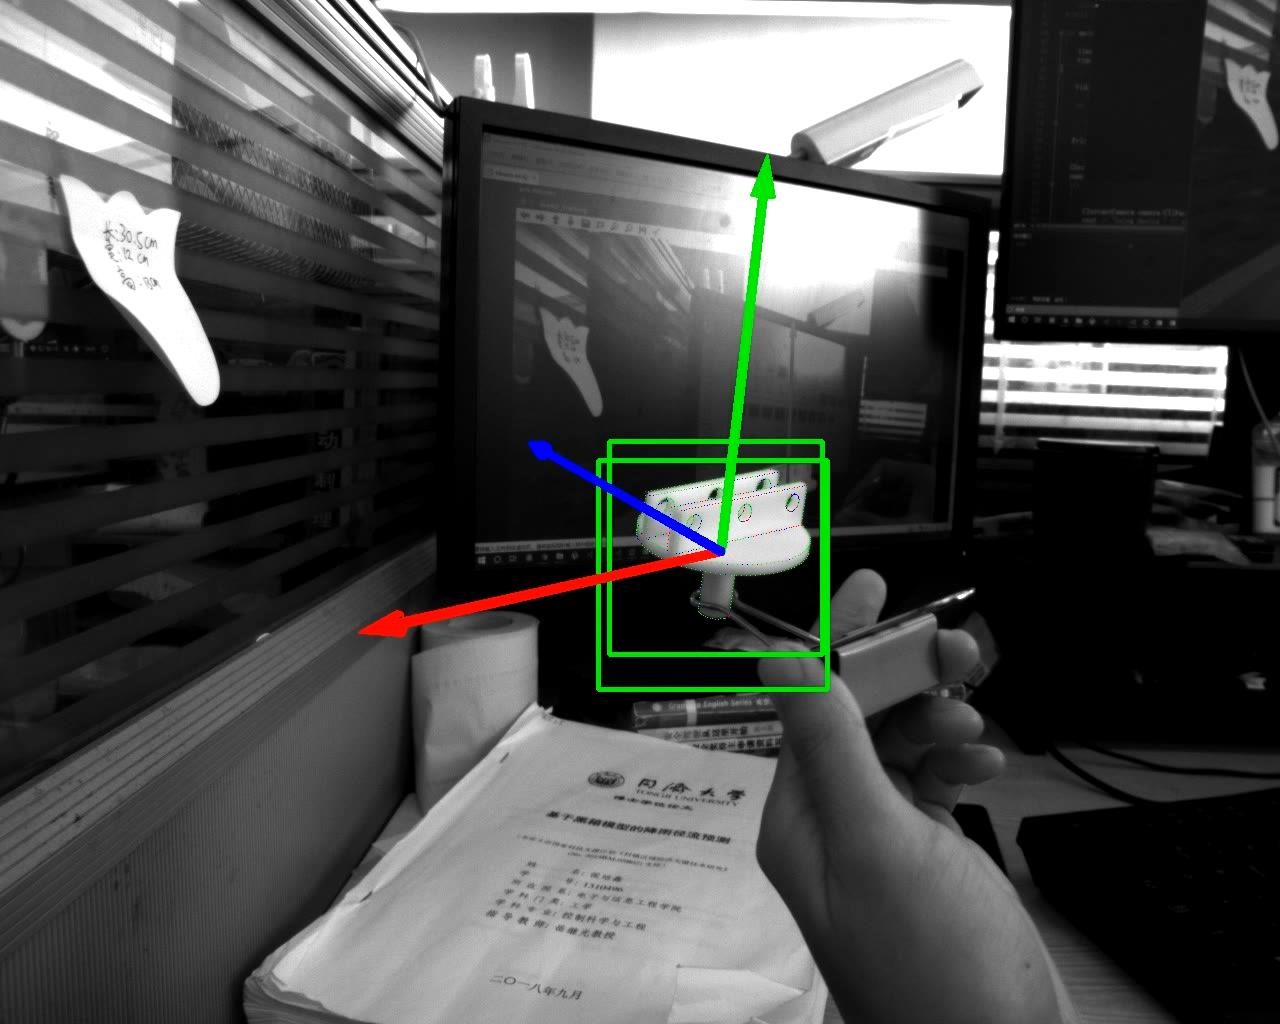
\includegraphics[height=3.8cm]{double_detec_pose2}
    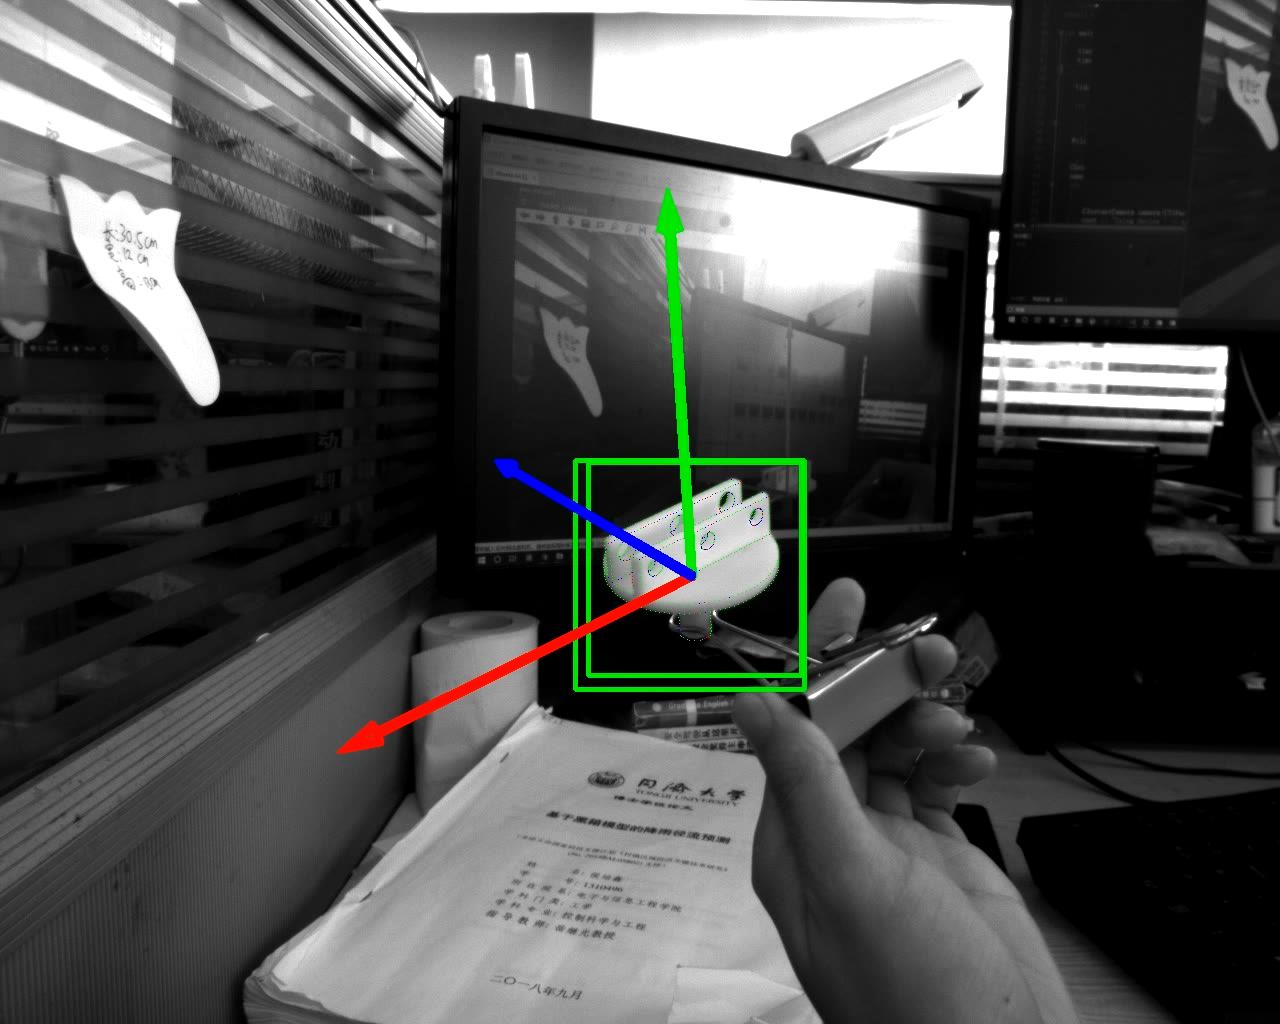
\includegraphics[height=3.8cm]{double_detec_pose3}
    \caption{多检情况的模板匹配结果}
    \label{fig:chap05:multi_pose_match}
    \end{figure}


\begin{figure}[t] %[h]
    \centering% 
        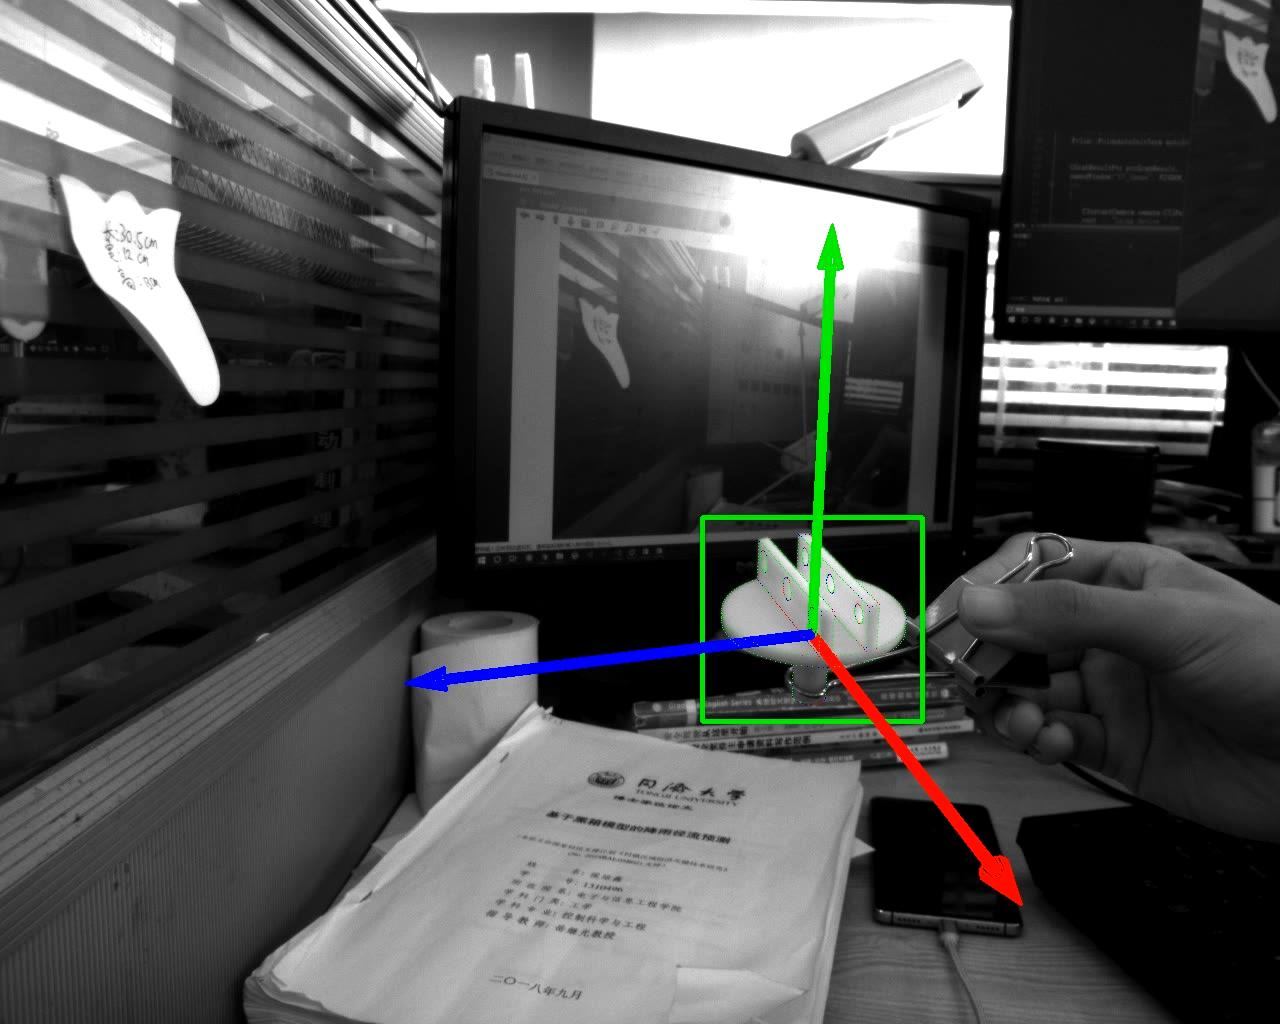
\includegraphics[height=3.8cm]{san_template_1}
        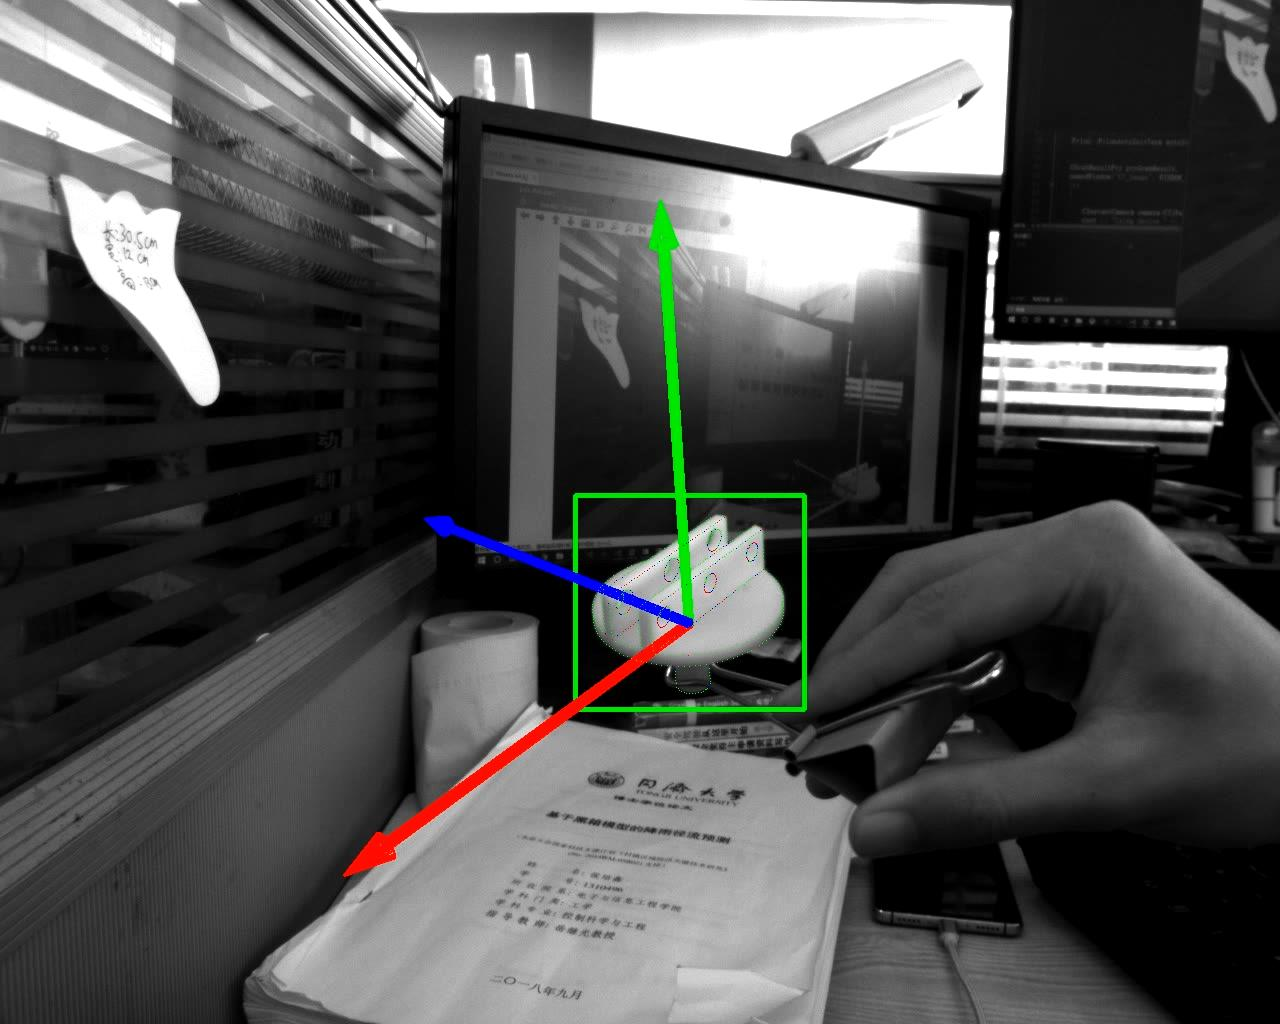
\includegraphics[height=3.8cm]{san_template_2}
        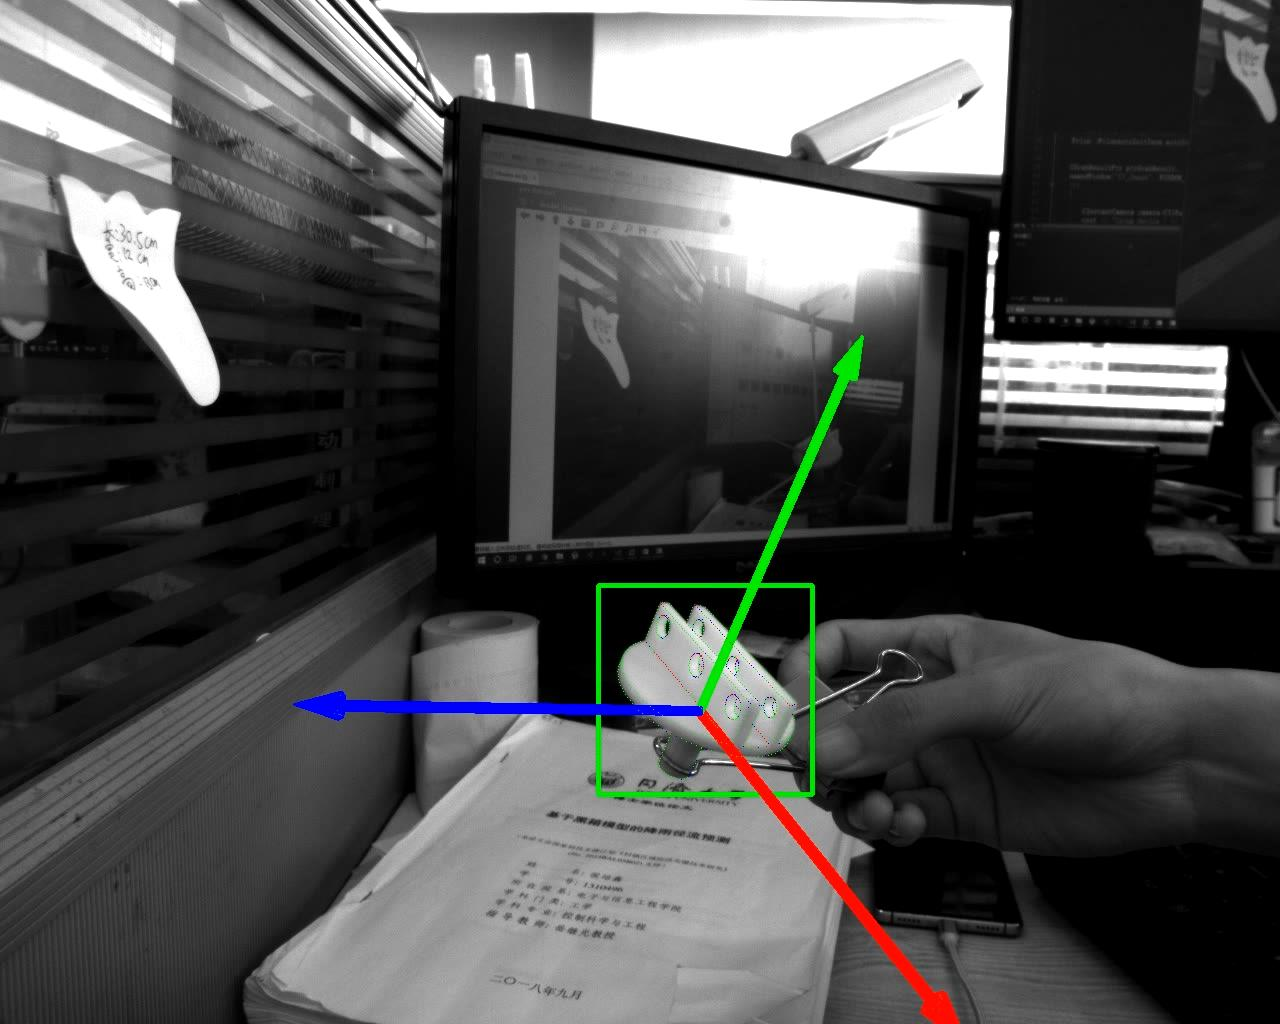
\includegraphics[height=3.8cm]{san_template_3}
        \vskip 1pt
        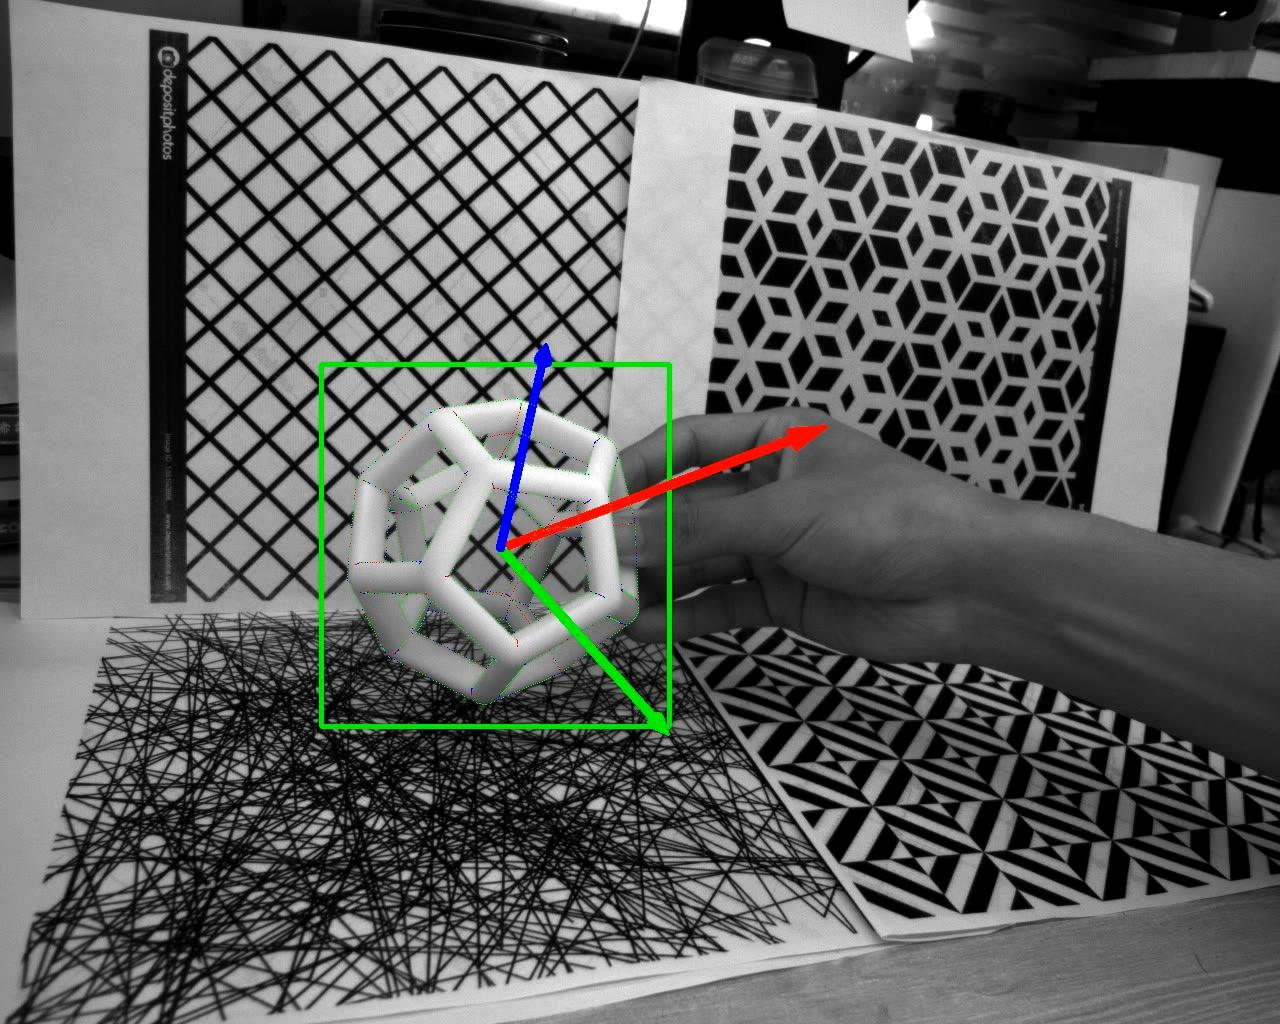
\includegraphics[height=3.8cm]{ball_template_1}
        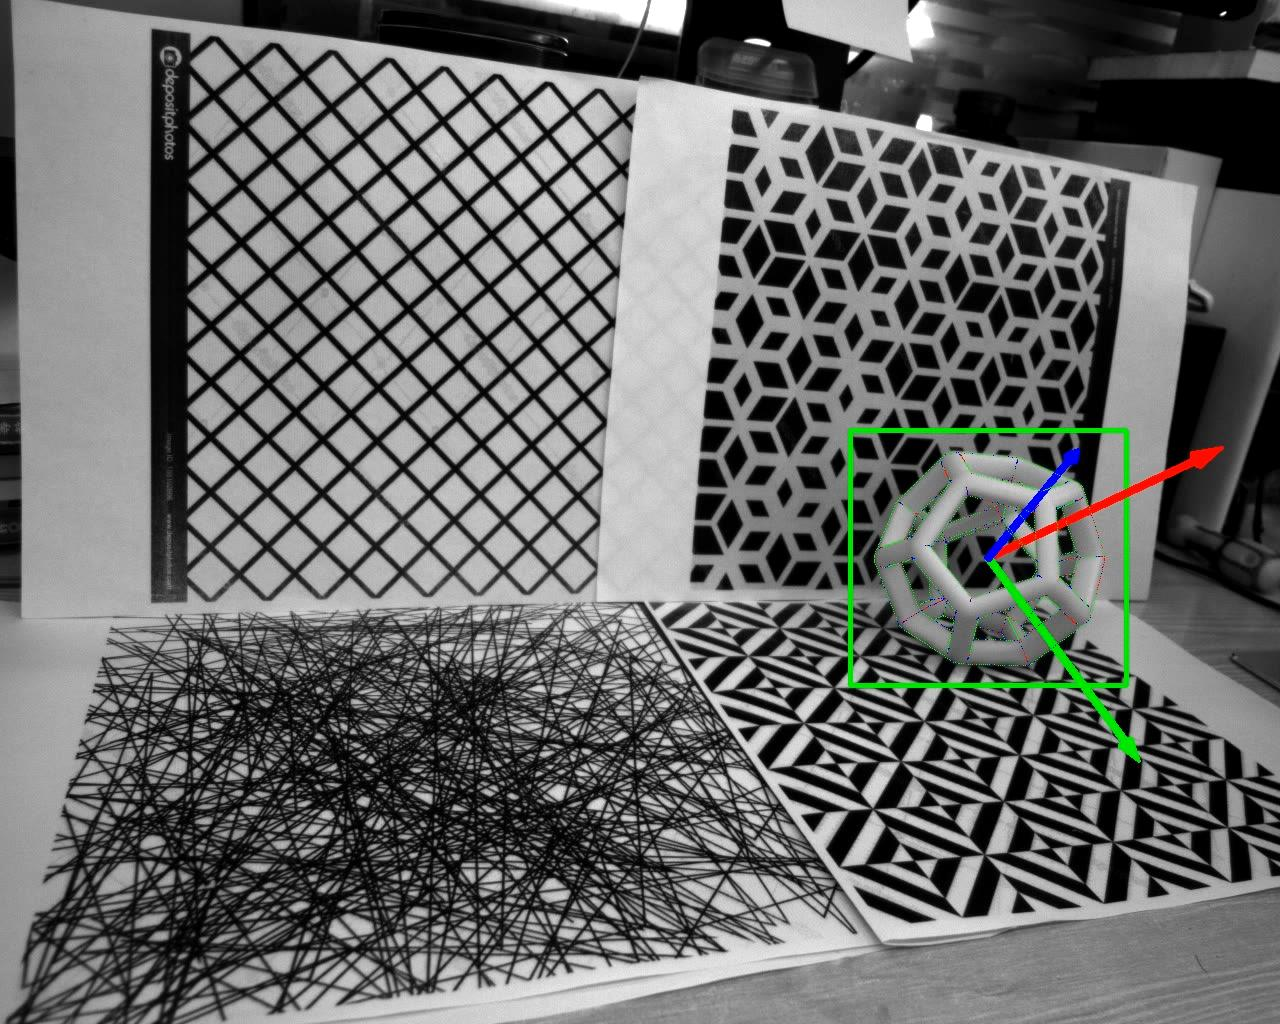
\includegraphics[height=3.8cm]{ball_template_2}
        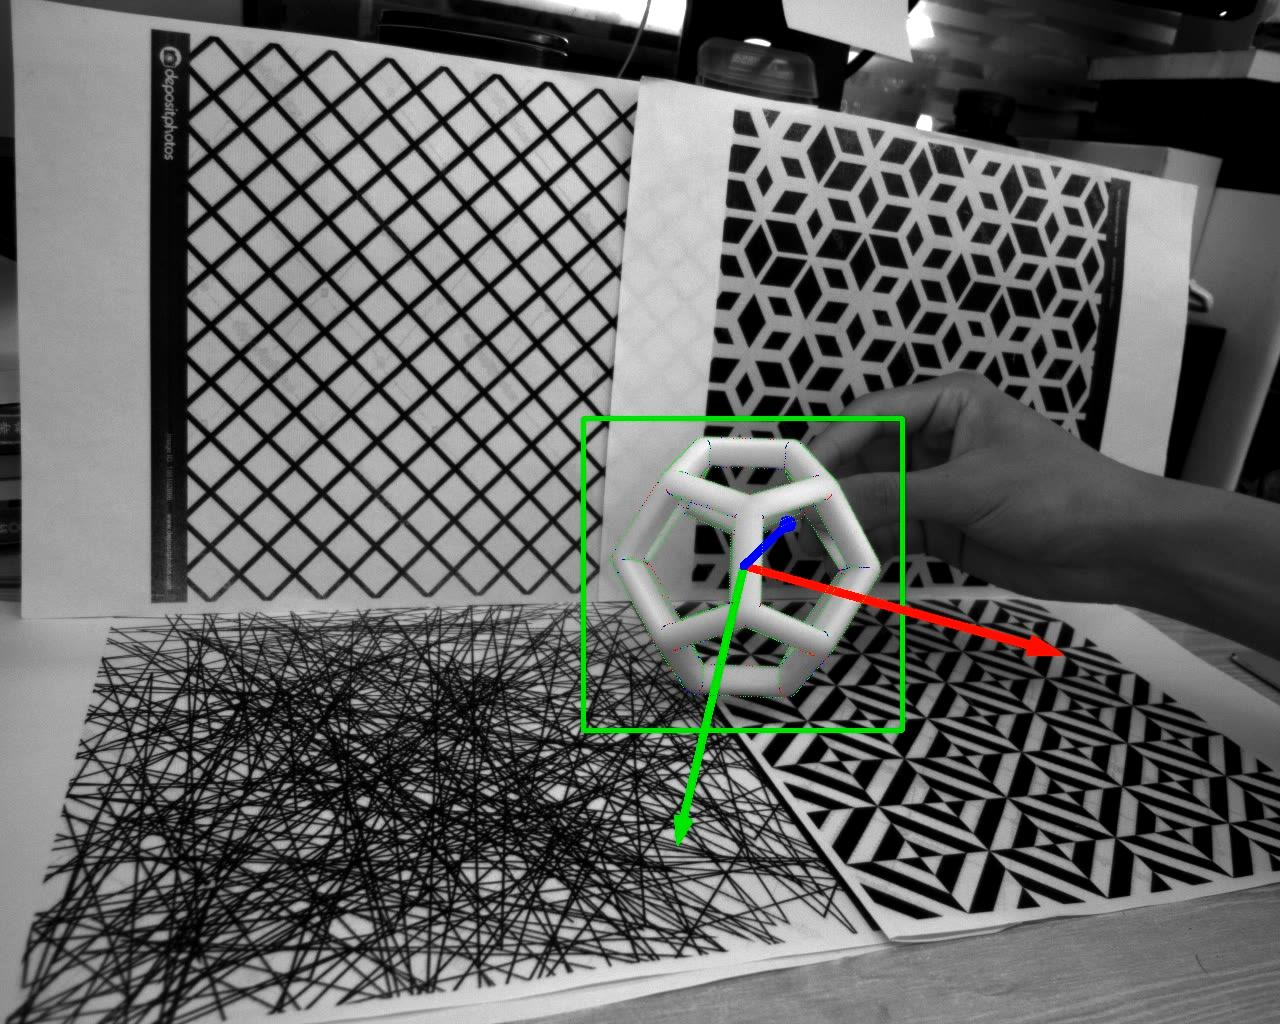
\includegraphics[height=3.8cm]{ball_template_3}
        \vskip 1pt
        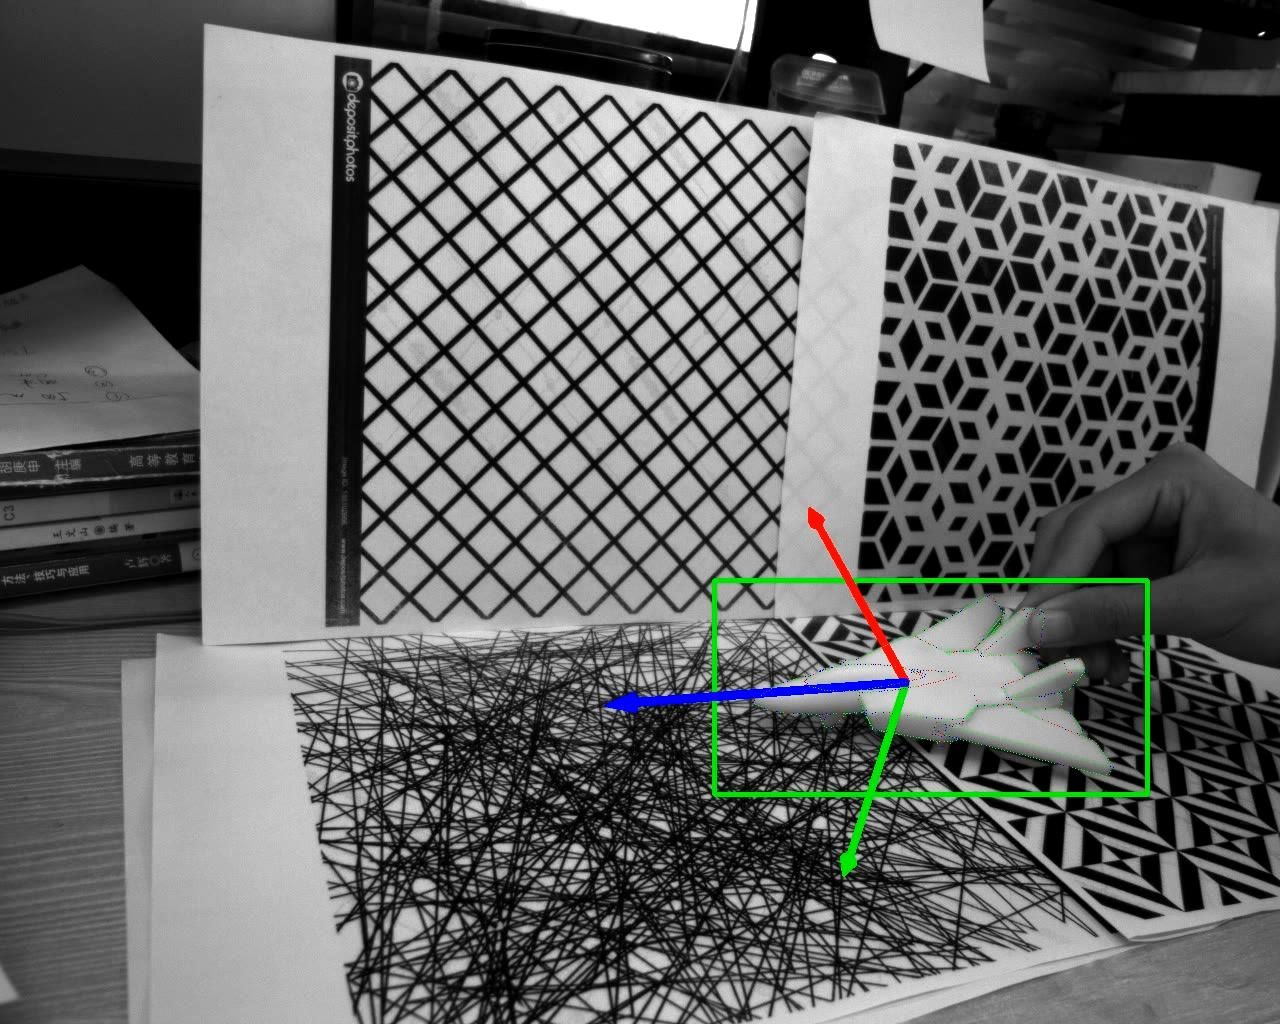
\includegraphics[height=3.8cm]{jet_template_1}
        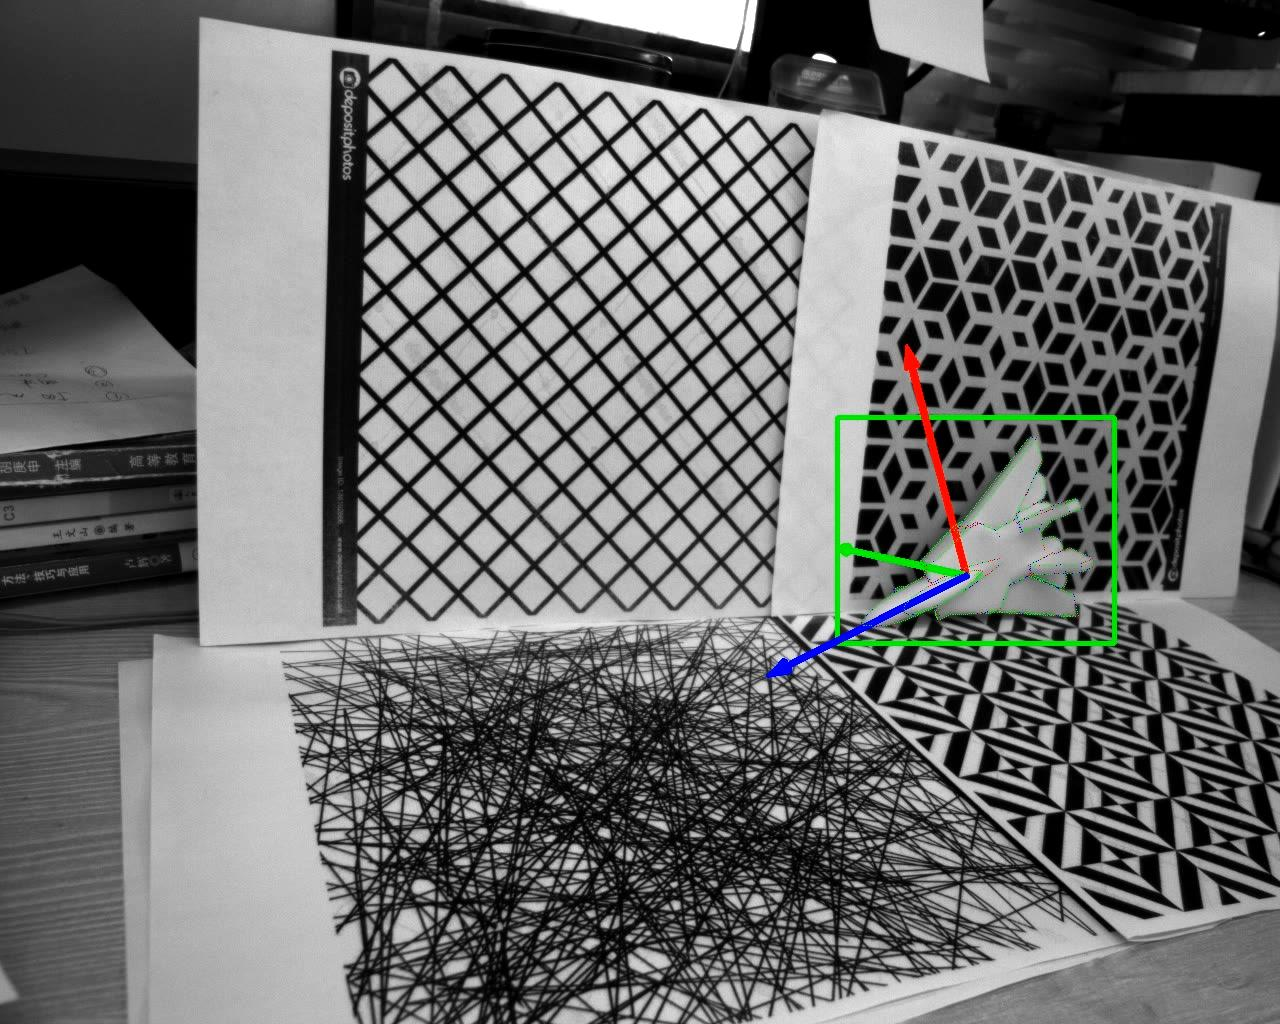
\includegraphics[height=3.8cm]{jet_template_2}
        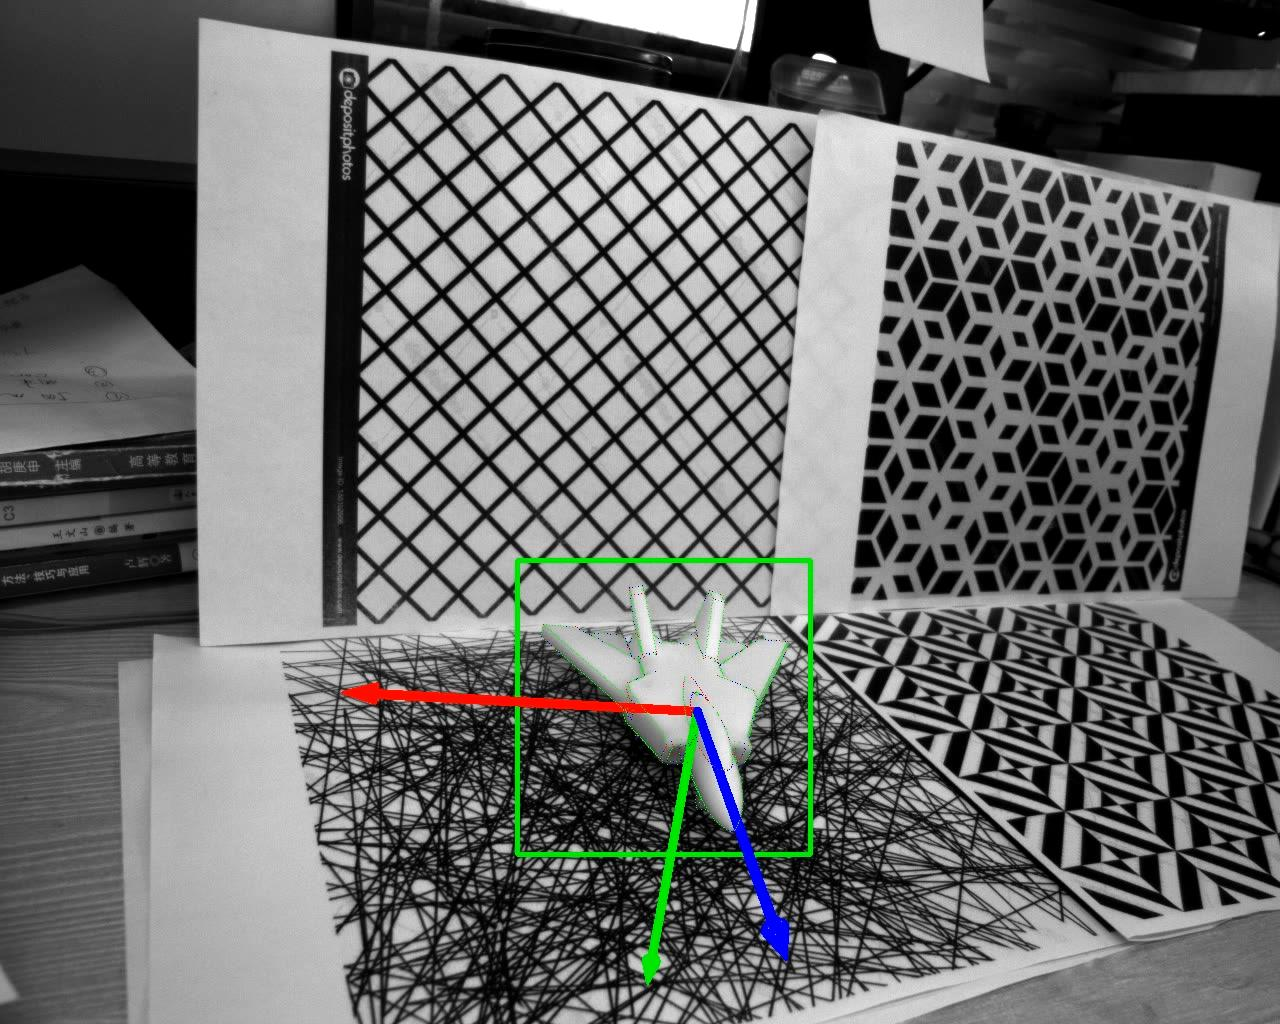
\includegraphics[height=3.8cm]{jet_template_3}
        \vskip 1pt
        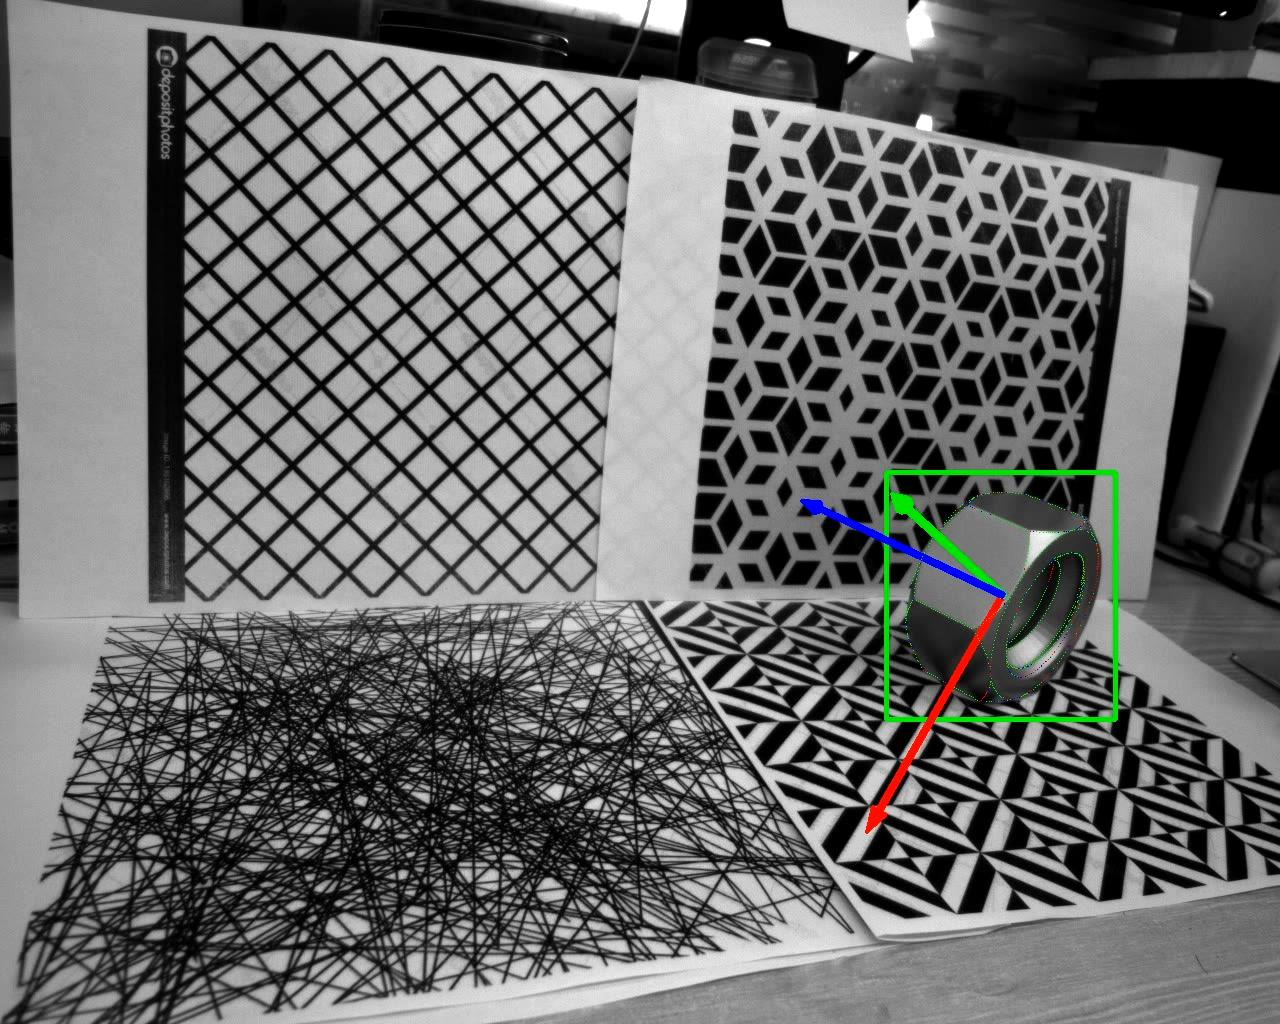
\includegraphics[height=3.8cm]{nut_template_1}
        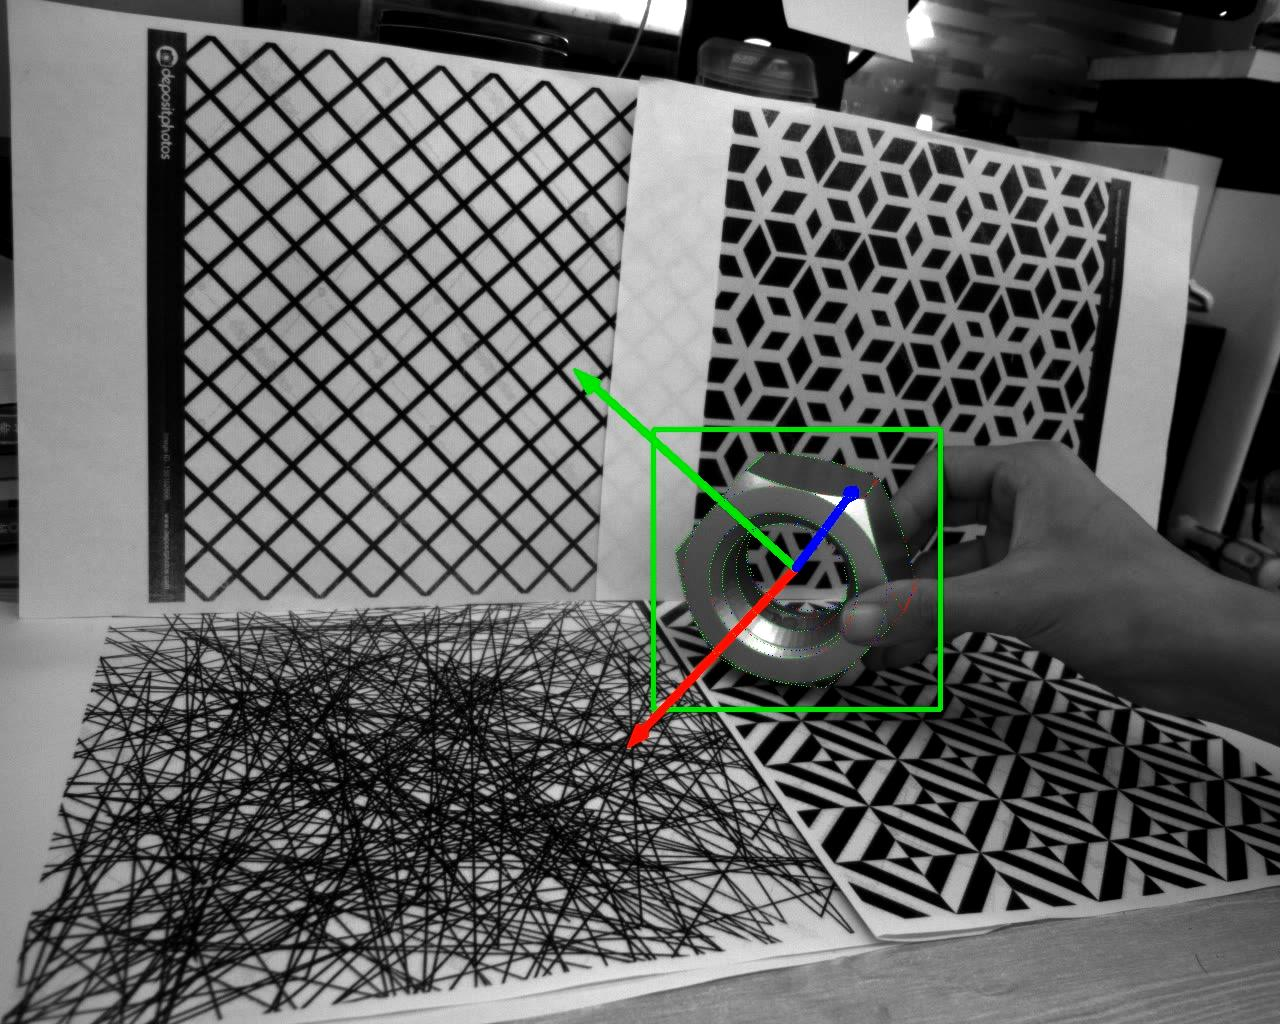
\includegraphics[height=3.8cm]{nut_template_2}
        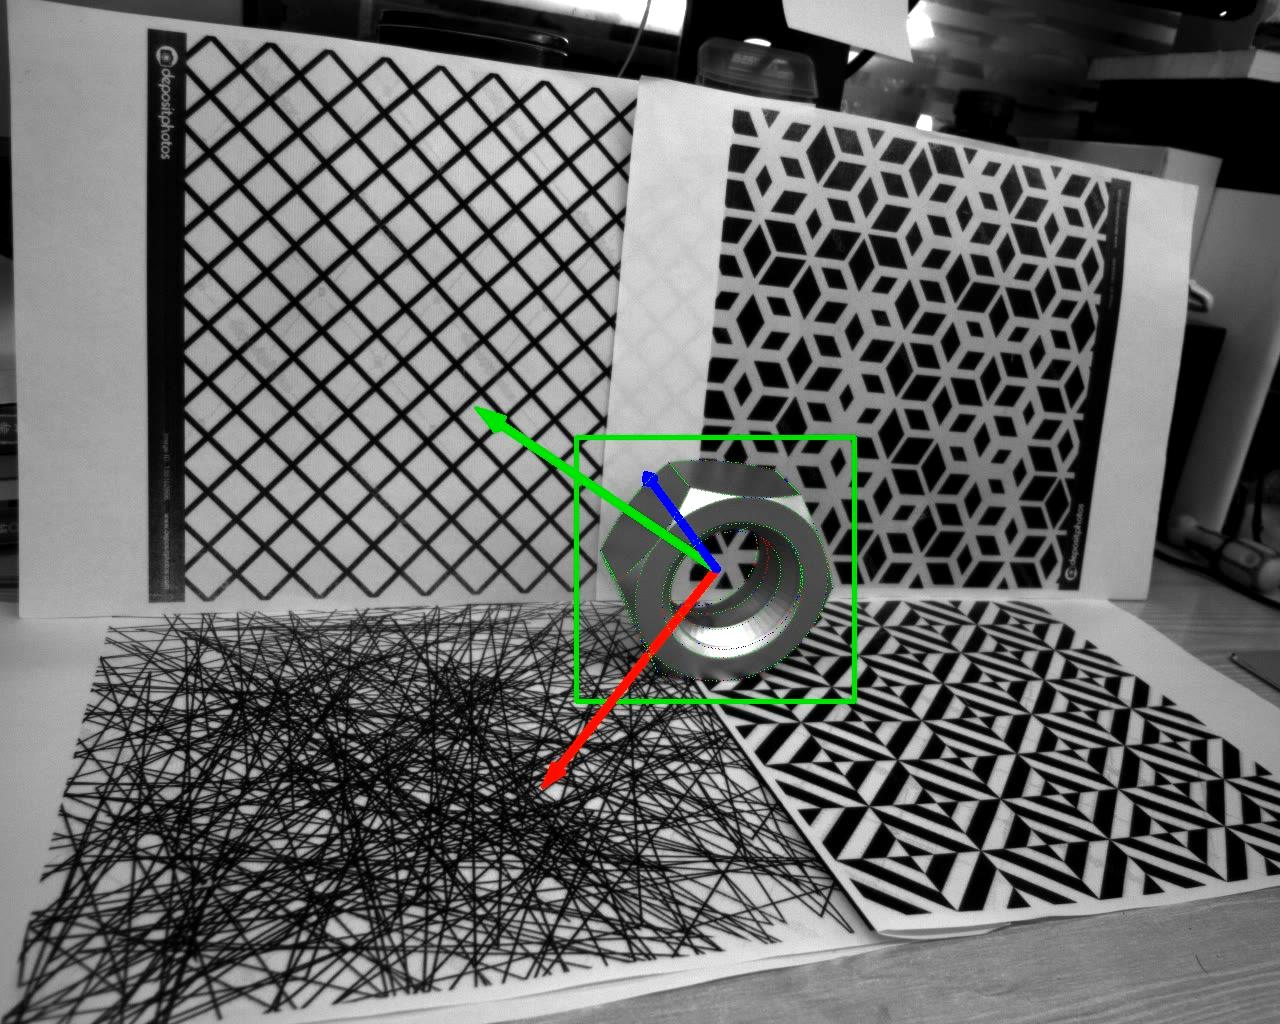
\includegraphics[height=3.8cm]{nut_template_3}
    \caption{模板匹配结果}
    \label{fig:chap05:pose_estimate_template_match}
    \end{figure}

\section{追踪系统测试}
\label{sec:track_test}
\subsection{实物场景测试}
\label{sec:real_video_test}
使用灰度相机采集的视频数据对追踪算法进行测试,以验证算法对复杂背景以及光照等干扰的鲁棒性。

\noindent{\textbf{背景测试}}
\begin{figure}[t] %[h]
    \centering%
    %%\subcaptionbox{目标物体图像区域\label{fig:chap03:area_interesting}}[\linewidth]{% 
    \subcaptionbox{测试背景\label{fig:chap05:bg_img_real}}{   
      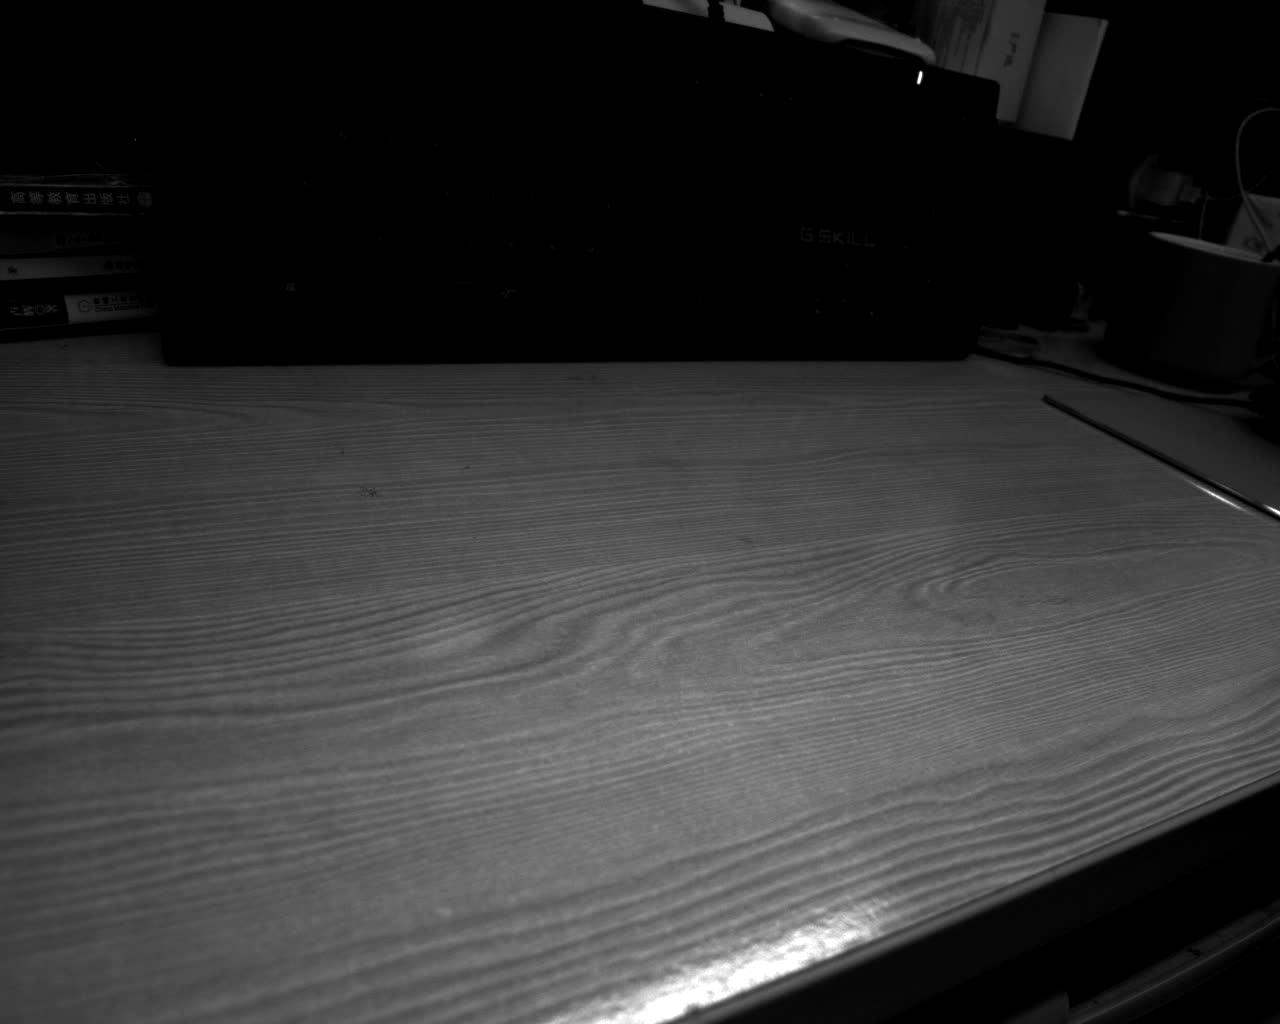
\includegraphics[height=3.8cm]{bg_r_1}
      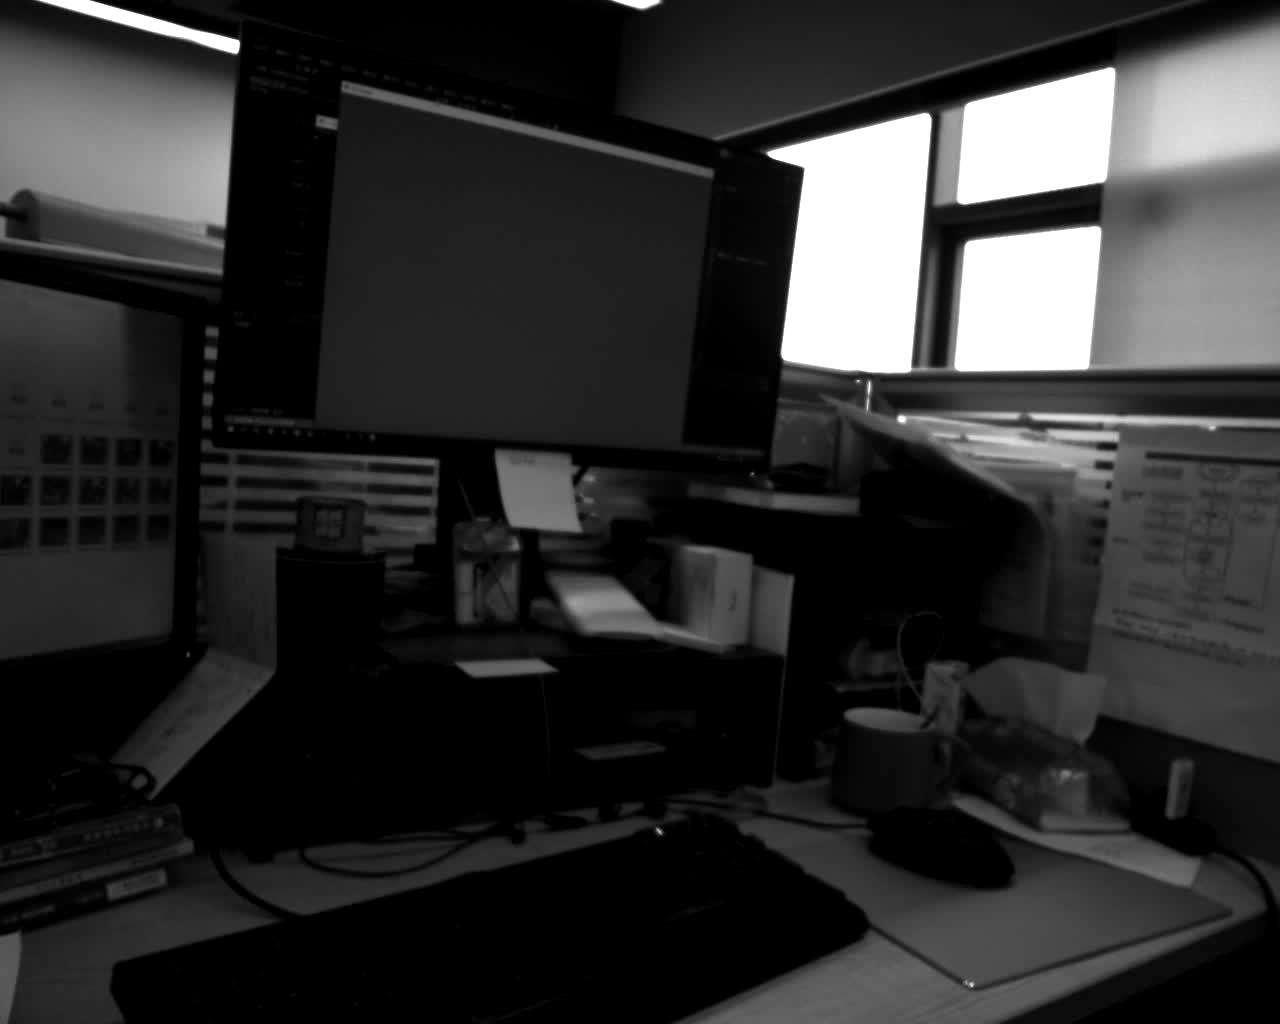
\includegraphics[height=3.8cm]{bg_r_2}
      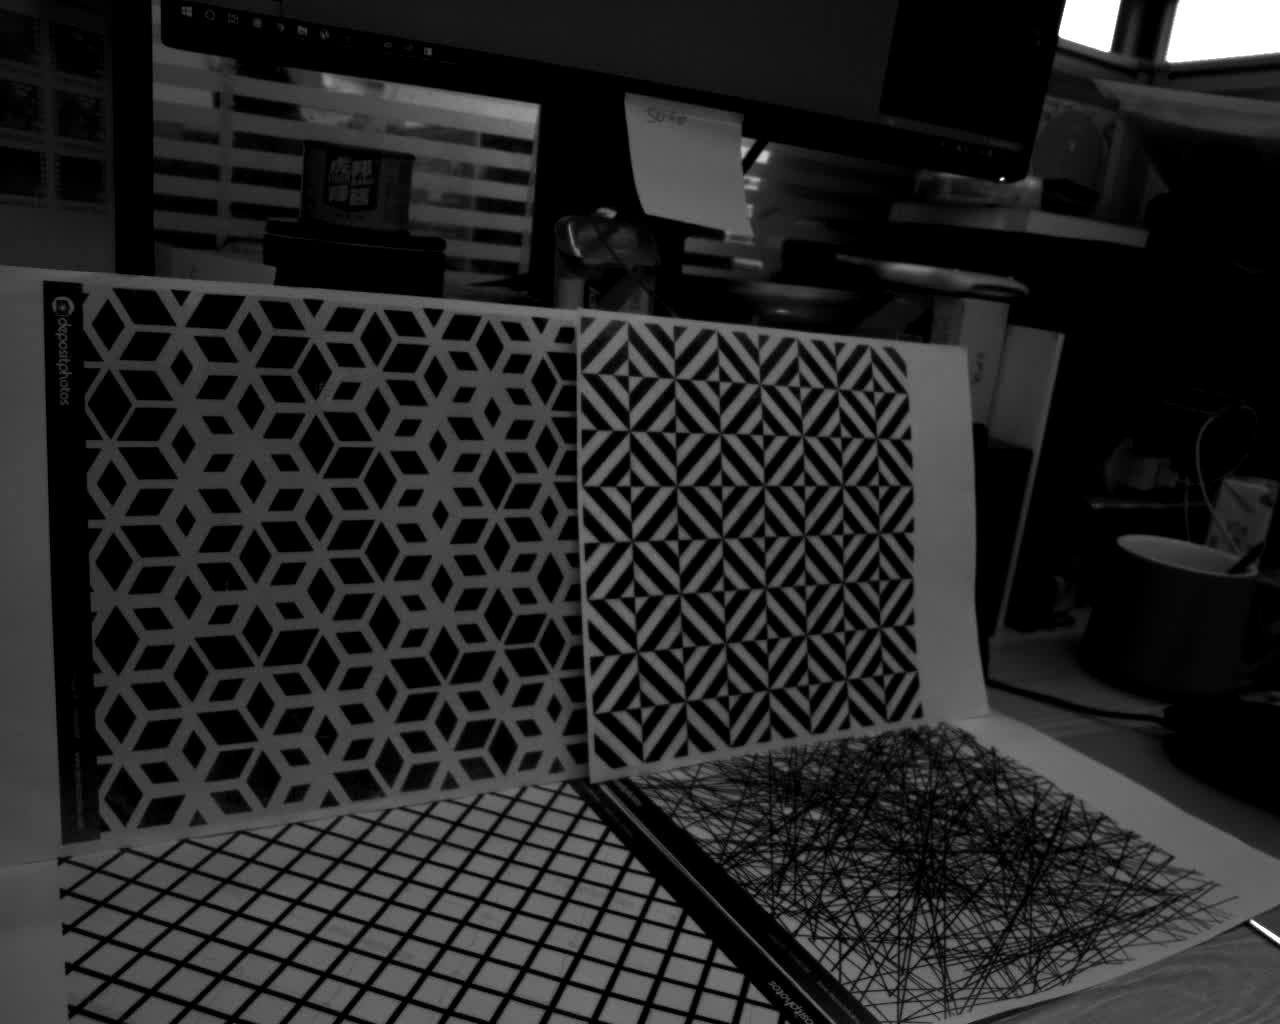
\includegraphics[height=3.8cm]{bg_r_3}}
      \vskip0.3cm
      \subcaptionbox{测试背景~DCM~张量图\label{fig:chap05:bg_img_real_dcm}}{
      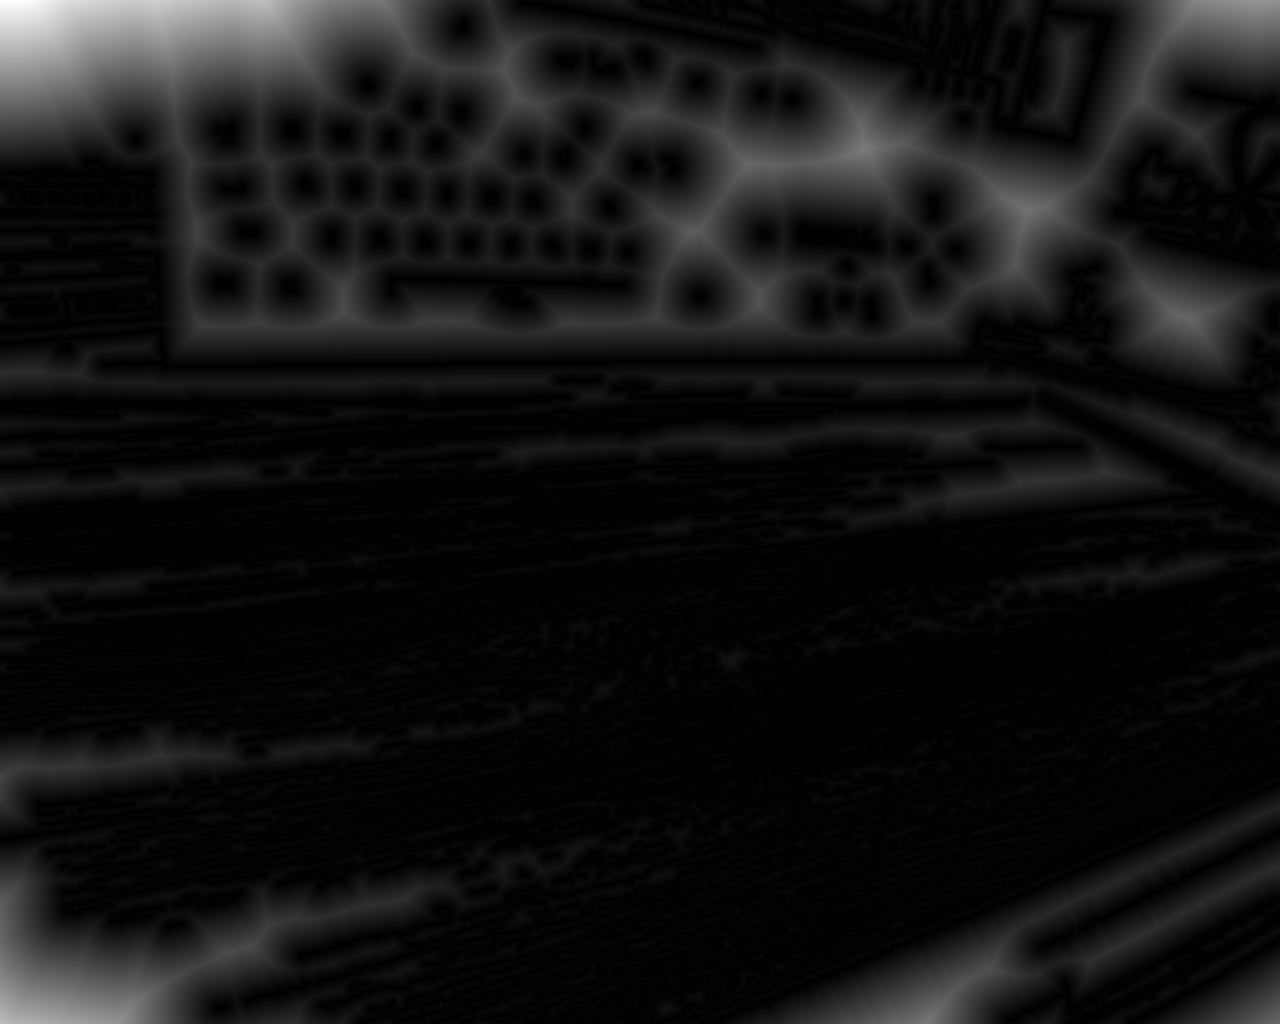
\includegraphics[height=3.8cm]{bg_r_dcm_1}
      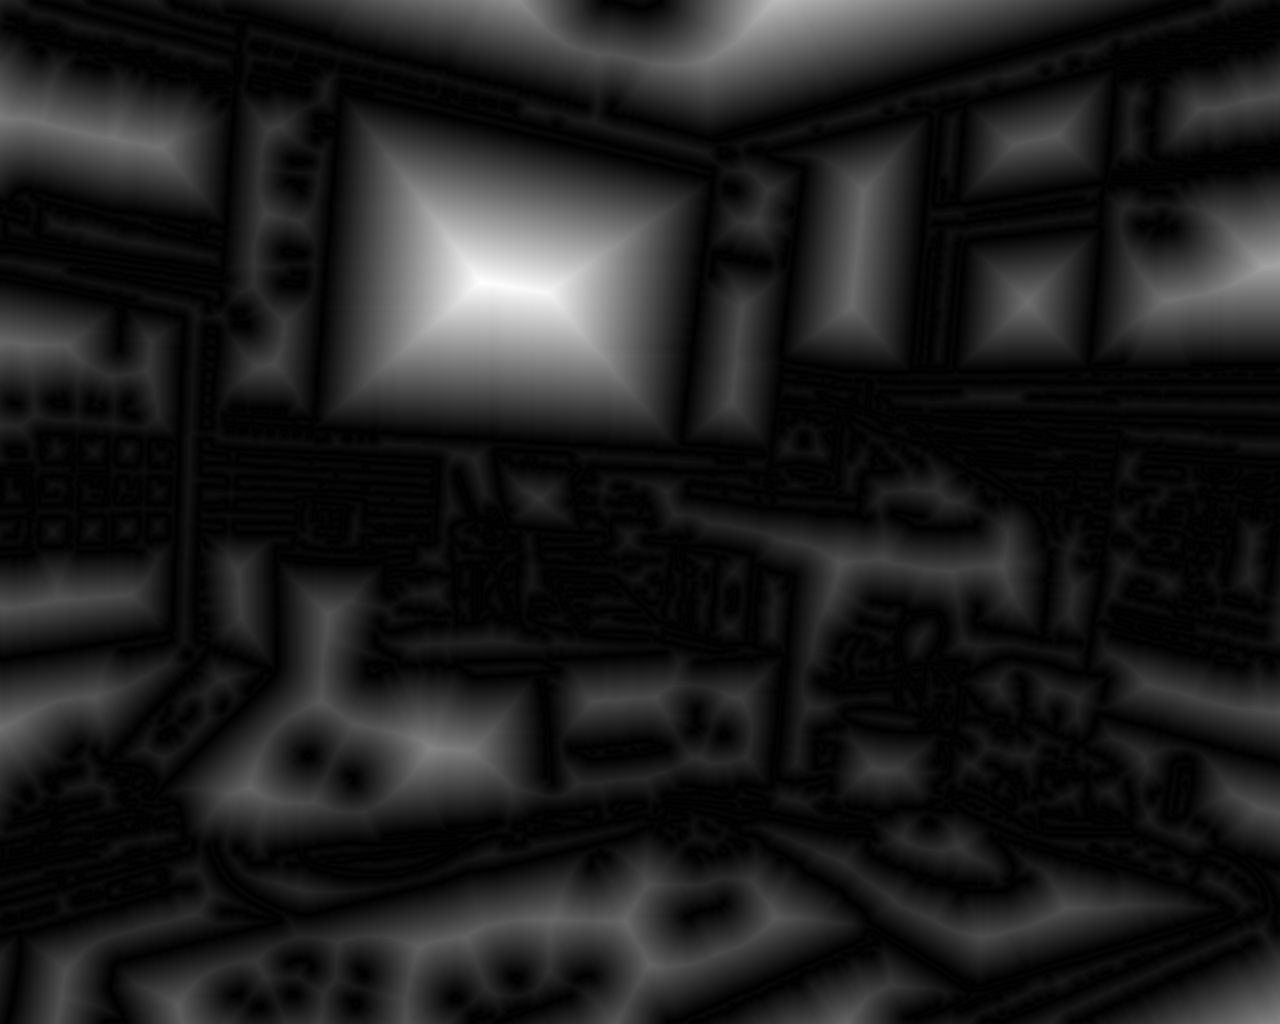
\includegraphics[height=3.8cm]{bg_r_dcm_2}
      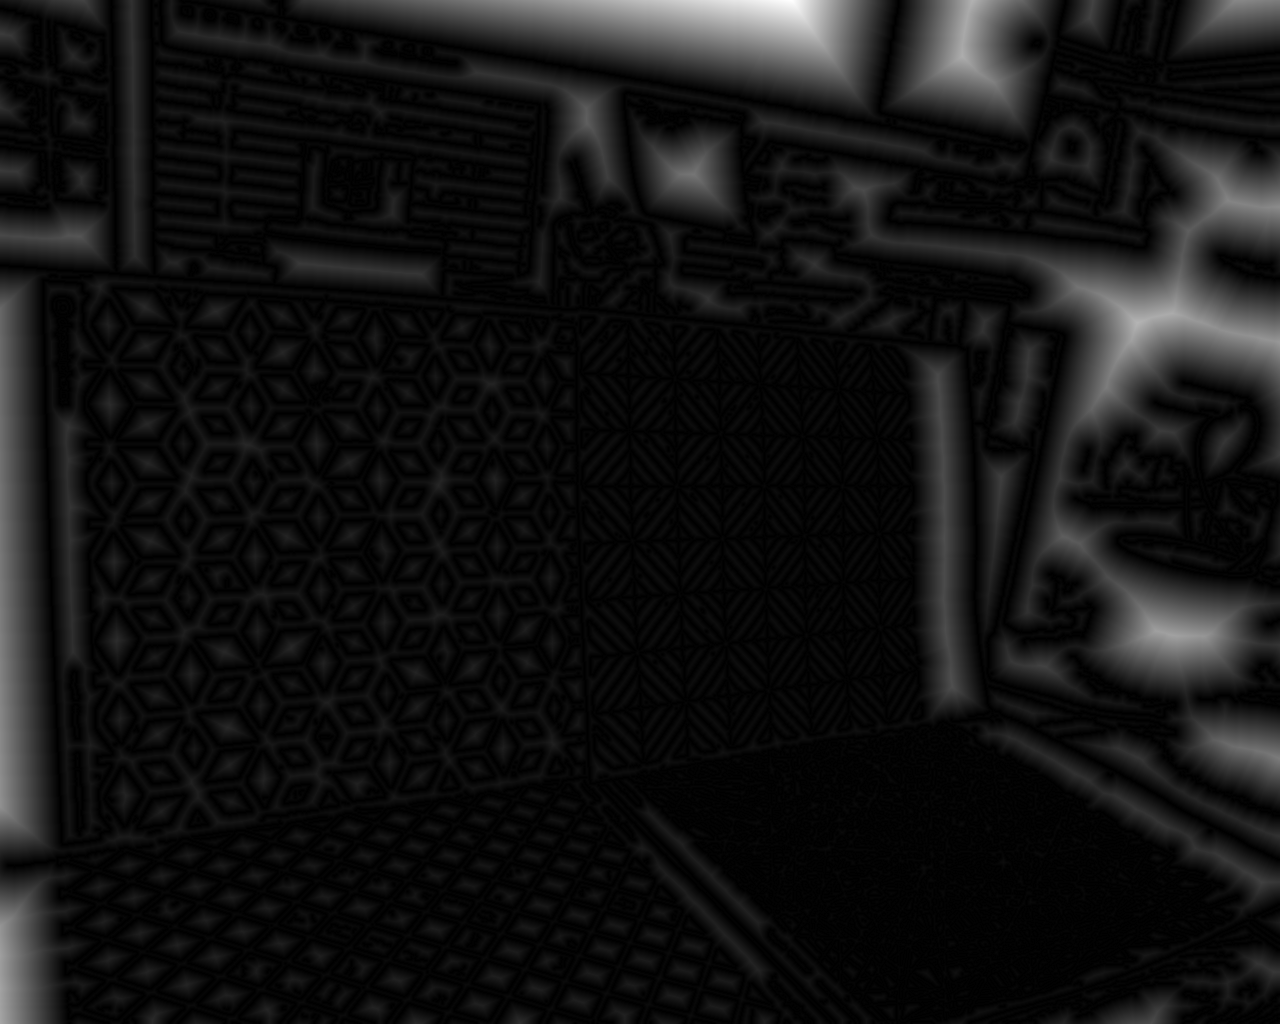
\includegraphics[height=3.8cm]{bg_r_dcm_3}}
    \caption{不同场景复杂度示意图}
    \label{fig:chap05:diff_bg_img}
    \end{figure}

追踪算法是通过寻找物体模型与场景边缘的最优匹配,以得到物体的位姿,因此场景的边缘复杂度直接影响
追踪算法的匹配难度,场景包含的边缘特征越复杂,则匹配的难度也就越高。因此为测试算法对不同背景的适应性,本文搭建了不同复杂度的场景,如图~\ref{fig:chap05:bg_img_real},
场景的~DCM~张量如图~\ref{fig:chap05:bg_img_real_dcm},背景的复杂度由左向右不断递增,在最右侧的场景中,本文通过寻找到的含有大量边缘信息的纹理图构建复杂背景。通过在不同场景中录制目标的运动视频以测试追踪算法,
所有视频的拍摄都在同一时间段的同一地点,相机的
光圈设置统一,以保证不同视频的亮度相似。由于背景的干扰主要影响光栅点的匹配,当出现与模型光栅点距离较近且方向相似
的背景边缘点时,算法有可能将模型匹配至背景边缘,导致误匹配。直观上,若背景中出现与模型边缘平行的背景边缘时,算法容易出现追踪失败,这对追踪算法的匹配精度以及整体寻优提出了更高的要求。

追踪的结果如图~\ref{fig:chap05:real_video_tracking}~所示,由图可知,在不同复杂度的背景干扰下,所有物体的追踪效果良好,模型光栅点匹配准确,三轴坐标系随物体位姿的变化精准,由此
证明追踪算法对背景干扰的鲁棒性高,能够适应不同场景复杂度、不同目标物体的位姿精确追踪。

\noindent{\textbf{亮度测试}}

在背景相同、目标物体相同的情况下,改变相机的光圈大小,以调整图像采集时的进光量,达到调节场景亮度的作用。通过该方法录制物体在不同亮度下的视频,以测试光照对算法的影响,结果如图~\ref{fig:chap05:light_change_test}~所示。
算法在不同亮度中追踪效果良好,但在亮度最高的图中,物体表面部分边缘由于过曝而无法分辨,导致相应的匹配光栅点得分较低,在图像中显示为红色点。在这类情况下,算法仅能够通过其余的部分物体轮廓确定其位姿。
产生过曝时,系统无法提取到物体的所有可见轮廓,导致追踪系统的稳定性比较差,因此在实际使用中应合理控制光源亮度,避免图像过曝。

\begin{figure}[t] %[h]
    \centering% 
        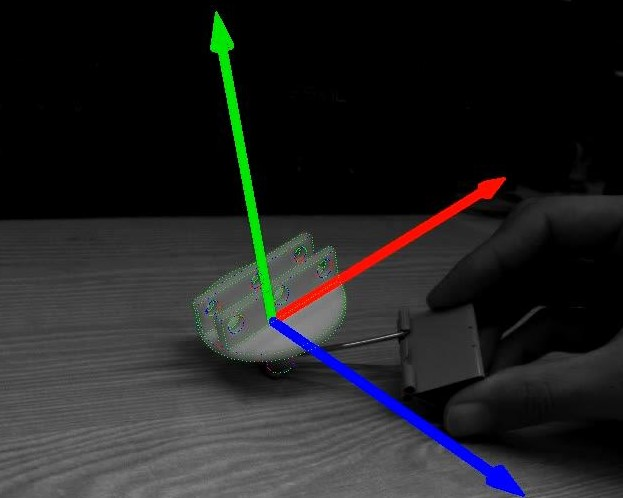
\includegraphics[height=3.8cm]{r_san_1}
        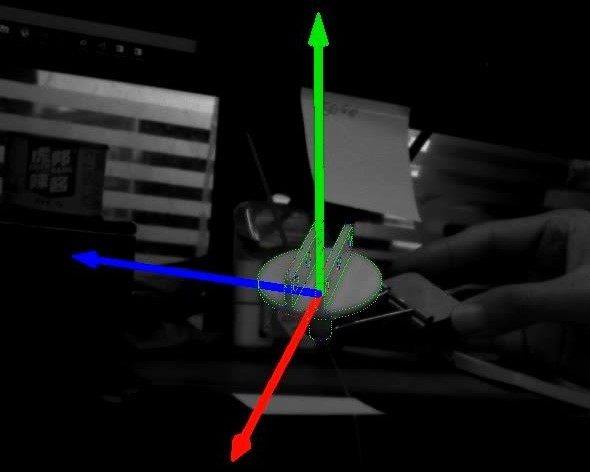
\includegraphics[height=3.8cm]{r_san_2}
        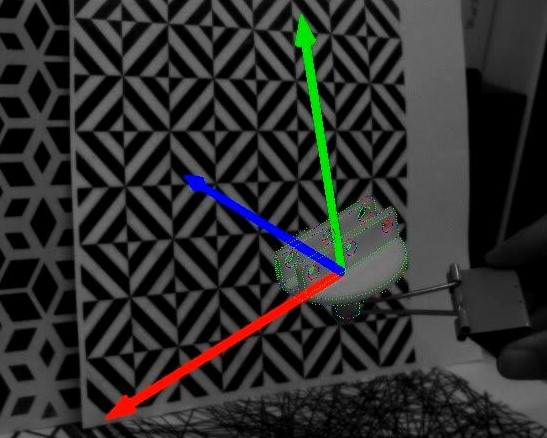
\includegraphics[height=3.8cm]{r_san_3}
        \vskip 1pt
        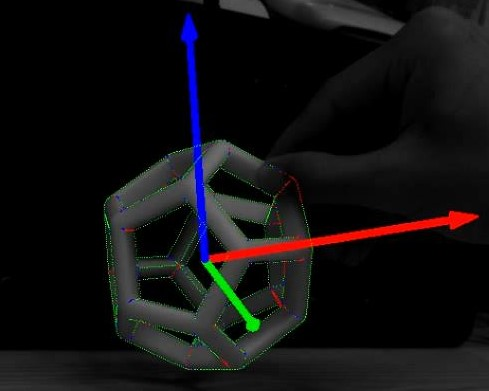
\includegraphics[height=3.8cm]{r_ball_1}
        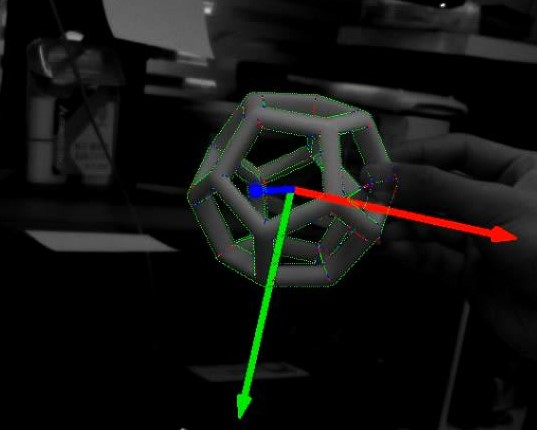
\includegraphics[height=3.8cm]{r_ball_2}
        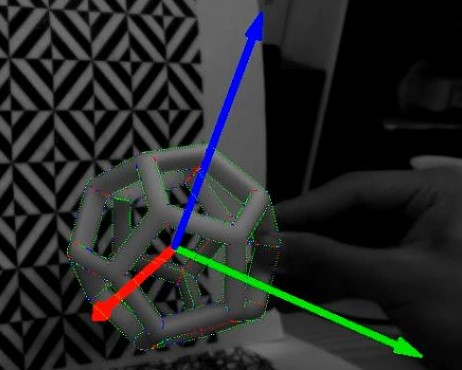
\includegraphics[height=3.8cm]{r_ball_3}
        \vskip 1pt
        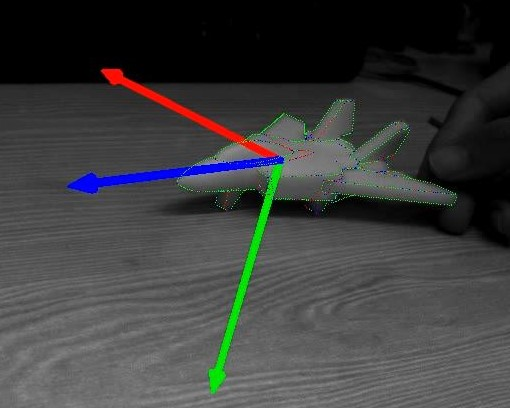
\includegraphics[height=3.8cm]{r_jet_1}
        \includegraphics[height=3.8cm]{r_jet_2}
        \includegraphics[height=3.8cm]{r_jet_3}
        \vskip 1pt
        \includegraphics[height=3.8cm]{r_nut_1}
        \includegraphics[height=3.8cm]{r_nut_2}
        \includegraphics[height=3.8cm]{r_nut_3}
    \caption{真实视频追踪结果}
    \label{fig:chap05:real_video_tracking}
    \end{figure}
    \begin{figure}[H] %[h]
        \centering%
            \includegraphics[height=2.8cm]{jet_light1_1}
            \includegraphics[height=2.8cm]{jet_light1_2}
            \includegraphics[height=2.8cm]{jet_light1_4}
            \includegraphics[height=2.8cm]{jet_guobao1}
            \vskip 1pt
            \includegraphics[height=2.8cm]{jet_light2_1}
            \includegraphics[height=2.8cm]{jet_light2_2}
            \includegraphics[height=2.8cm]{jet_light2_4}
            \includegraphics[height=2.8cm]{jet_guobao2}
        \caption{场景亮度变化及过曝示意图}
        \label{fig:chap05:light_change_test}
        \end{figure}

\subsection{公开数据集及~CG~渲染视频测试}
\label{sec:cg_video_open_dataset_test}
使用公开数据集以及章节~\ref{sec:dataset_engine}~中构建的~CG~渲染数据库对追踪算法的精度进行定量测试。

\noindent{\textbf{公开数据集}}

本文使用公开数据库~Rigid Pose\cite{PauwelsRealTimeModelBasedRigid2013}~对算法的精度进行测试。该数据库是以真实场景作为背景,而将目标物体通过渲染的方式叠加在真实环境中,进而通过渲染引擎控制
物体的运动并保存其位姿真实。该数据库包含~6~种物体的运动视频以及真值数据,其中~clown~模型是表面无纹理且结构较为复杂的物体,相比其他模型更适合作为本文的测试目标。使用本文所研究的
追踪算法对~Clown\_800\_noise\_free~视频中的~clown~模型进行位姿追踪,效果如图~\ref{fig:chap05:rigidpose_track}~所示,追踪的数据与真值的对比如图~\ref{fig:chap05:rigidpose_rig_track}~所示。

由于物体模型复杂,且运动速度较快,因此对该数据库的追踪难度较大。本文所提算法能够完成对该物体的位姿追踪,并且精度较高,仅在物体位姿发生较大变化时存在一定的追踪迟滞现象,但整体跟随效果
良好。存在迟滞的原因是物体表面部分边缘在图像中难以分辨,导致算法将某些边缘点的权重降得过低,匹配不及时。追踪过程中能够采集到的模型细节信息较少,因此在物体位姿发生较小变化时,物体边缘的变化不明显,
但在边缘出现较大变化后,算法又能够精确地在图像中配准模型,实现准确的位姿追踪。

\begin{figure}[b] %[h]
    \centering% 
      \includegraphics[height=3.6cm]{rigid_1}
      \includegraphics[height=3.6cm]{rigid_4}
      \includegraphics[height=3.6cm]{rigid_3}
      \vskip 1pt
      \includegraphics[height=3.6cm]{rigid_8}
      \includegraphics[height=3.6cm]{rigid_7}
      \includegraphics[height=3.6cm]{rigid_6}
      %\vskip 1pt
      %\includegraphics[height=3.6cm]{rigid_7}
      %\includegraphics[height=3.6cm]{rigid_8}
      %\includegraphics[height=3.6cm]{rigid_9}
    \caption{Rigid Pose追踪效果图}
    \label{fig:chap05:rigidpose_track}
    \end{figure}


    \begin{sidewaysfigure}
        \centering
        \subcaptionbox{x轴旋转\label{fig:chap05:rx}}{
        \includegraphics[width=0.31\textwidth]{rp_rx}}\hspace{0.1em}
        \subcaptionbox{y轴旋转\label{fig:chap05:ry}}{
        \includegraphics[width=0.31\textwidth]{rp_ry}}\hspace{0.1em}
        \subcaptionbox{z轴旋转\label{fig:chap05:rz}}{
        \includegraphics[width=0.31\textwidth]{rp_rz}}
        \vskip 0.3cm
        \subcaptionbox{x轴平移\label{fig:chap05:tx}}{
        \includegraphics[width=0.31\textwidth]{rp_tx}}\hspace{0.1em}
        \subcaptionbox{y轴平移\label{fig:chap05:ty}}{
        \includegraphics[width=0.31\textwidth]{rp_ty}}\hspace{0.1em}
        \subcaptionbox{z轴平移\label{fig:chap05:tz}}{
        \includegraphics[width=0.31\textwidth]{rp_tz}}
        \caption{Rigid Pose追踪精度测试图}
        \label{fig:chap05:rigidpose_rig_track}
    \end{sidewaysfigure}

Pauwels\cite{PauwelsRealTimePoseDetection2016}~等人提出的追踪算法同样在该数据集中进行了精度测试,本文将所提算法与其进行了精度对比,结果如表~\ref{table:chap05:tracking_methods_error}~所示。本文追踪算法在~clown~数据集上的角度追踪平均误差为~$1.835^\circ$,平移向量
平均误差为~0.989mm~,相比~Pauwels~等人所提的稀疏点追踪方法,优势明显;而与深度稠密追踪算法相比,仅在平移向量误差上稍大,但本文算法仅使用灰度图像,在算法复杂度以及计算耗时上有较大优势。根据测试对比,本文所提
算法在同等设备条件下相比稀疏点集追踪算法精度高,其精度水平已经达到使用深度相机的稠密点集追踪方法。

\begin{table}[t]
    \begin{minipage}[c]{0.3\linewidth}
        \centering
        \captionof{table}{追踪算法平均误差}
        \label{table:chap05:tracking_methods_error}
           \begin{tabular}{lcl}
               \toprule
               Methods & $R(^\circ)$ & $\textrm{T}(\textrm{mm})$   \\
               \midrule
               Sparse   & 3.112 & 1.521\\ 
               Dense    & 2.243 & \textbf{0.953}\\ 
               Ours    & \textbf{1.835} & 0.989\\ 
               \bottomrule
           \end{tabular}
    \end{minipage}
    \hfill
    \begin{minipage}[c]{0.3\linewidth}
        \centering
        \captionof{table}{不同背景追踪精度}
        \label{table:chap05:chagne_background}
           \begin{tabular}{ccl}
               \toprule
               Background & $R(^\circ)$ & $\textrm{T}(\textrm{mm})$   \\
               \midrule
               1   & 0.846 & 0.655\\ 
               2    & 0.824 & 0.647\\ 
               3    & 0.852 & 0.662\\ 
               \bottomrule
           \end{tabular}
    \end{minipage}
    \hfill
    \begin{minipage}[c]{0.3\linewidth}
        \centering
        \captionof{table}{不同尺度追踪精度}
         \label{table:chap05:cg_track_jdu}
            \begin{tabular}{lcl}
                \toprule
                Scale(Pix) & $R(^\circ)$ & $\textrm{T}(\textrm{mm})$   \\
                \midrule
                129   & 1.254 & 0.844\\ 
                213    & 0.873 & \textbf{0.613}\\ 
                321    & \textbf{0.846} & 0.655\\ 
                \bottomrule
            \end{tabular}
      \end{minipage}%
  \end{table}
  \begin{figure}[t] %[h]
    \centering%
      \includegraphics[height=3.6cm]{cg_bg1}
      \includegraphics[height=3.6cm]{cg_bg2}
      \includegraphics[height=3.6cm]{cg_bg3}
    \caption{不同背景目标追踪}
      \label{fig:chap05:diff_back_track}
  \end{figure}
  \begin{figure}[t] %[h]
    \centering%
      \includegraphics[height=3.6cm]{cg_scale1}
      \includegraphics[height=3.6cm]{cg_scale2}
      \includegraphics[height=3.6cm]{cg_scale3}
    \caption{不同尺度目标追踪}
      \label{fig:chap05:scale_track_res}
  \end{figure}
  \noindent{\textbf{CG~渲染数据集}}

通过渲染得到的视频及其位姿真值对算法的追踪精度进行测试。首先测试物体对不同背景的追踪精度,在渲染测试视频时,相机的轨迹以及场景光照完全相同,在每帧图像中仅物体所在的背景图案存在变化。追踪效果如图~\ref{fig:chap05:diff_back_track}~所示,算法能够在不同背景下对目标实现精确追踪。
在三种背景下对飞机模型实现追踪的精度如表~\ref{table:chap05:chagne_background}~所示,实验结果与真实场景的测试结果相同,再一次证明了匹配寻优算法的精确性,在追踪过程中出现与物体模型边缘平行的背景边缘时,算法能够通过解目标函数的最小值以正确匹配物体边缘,有效降低背景对追踪算法的影响。
因此在不同背景下,平均角度误差以及平均平移向量误差基本不变,算法对背景扰动的鲁棒性强。

测试中发现算法追踪精度受物体在图像中的尺寸影响较大,本文通过调整相机与物体的距离,测试不同情况下的追踪精度,实验结果如图~\ref{fig:chap05:scale_track_res}~所示,追踪角度如表~\ref{table:chap05:cg_track_jdu}。
实验结果表明物体在图像中的尺度越大,追踪精度越高,尺度越小,追踪精度越低,这是由于相机距离物体较近时,物体在图片中所占的像素数量较多,使得物体边缘提取更加明显,而物体距离相机较远时,用于表现物体特征的像素减少,提取到的有效边缘也随之减少,导致精度有所下降。
因此在实际使用时,要分析目标物体在相机中的成像尺寸,或者选用更高分辨率的相机以满足追踪的精度要求。



\subsection{遮挡情况测试}
\label{sec:obst_test}
本节将测试章节~\ref{sec:Weight optimization algorithm}~中提出的自适应权重优化算法,该算法通过降低被遮挡边缘的优化权重,使得配准过程趋向于未被遮挡的部分,通过该方法以提高追踪系统的鲁棒性。

首先测试算法对被遮挡边缘的判别效果,本文所提算法通过模型边缘方向与图像的边缘方向计算光栅点的权重,当两者夹角接近~$n\pi~(n=0,1,2,\dotsc)$~时,认为匹配良好,则将该光栅点权重设置较高;若两者夹角接近~$\frac{\pi}{2}+n\pi~(n=0,1,2,\dotsc)$~时,认为匹配较差,则将该光栅点权重设置较低。
如图~\ref{fig:chap05:point_weight_cal}~所示为遮挡情况下的光栅点权重计算结果,图中使用三种颜色以表示不同光栅点的权重范围,其中绿色点为匹配良好的点,其权重大于~$0.8$,红色点为匹配误差较大的点,其权重低于~$0.3$,其余为蓝色点,权重为~$0.3\sim 0.8$。
通过方向夹角的计算,算法能够正确判断物体边缘中被遮挡的部分,及时降低被遮挡边缘的优化权重。

\begin{figure}[t] %[h]
    \centering% 
      \includegraphics[height=3.77cm]{quan_ball_1}
      \includegraphics[height=3.77cm]{quan_jet_1}
      \includegraphics[height=3.77cm]{quan_nut_1}
      \vskip 1pt
      \includegraphics[height=3.77cm]{quan_ball_2}
      \includegraphics[height=3.77cm]{quan_jet_2}
      \includegraphics[height=3.77cm]{quan_nut_2}
    \caption{光栅点权重计算}
    \label{fig:chap05:point_weight_cal}
    \end{figure}

    \begin{figure}[t] %[h]
        \centering%
        \subcaptionbox{原始追踪算法\label{fig:chap05:zhedang_yuanshi}}{   
          \includegraphics[height=3.8cm]{zhedang_bad_1}
          \includegraphics[height=3.8cm]{zhedang_bad_2}
          \includegraphics[height=3.8cm]{zhedang_bad_3}}
          \vskip0.3cm
          \subcaptionbox{改进后的追踪算法\label{fig:chap05:zhedang_gaijin}}{
          \includegraphics[height=3.8cm]{zhedang_nice_1}
          \includegraphics[height=3.8cm]{zhedang_nice_2}
          \includegraphics[height=3.8cm]{zhedang_nice_3}}
        \caption{遮挡情况追踪结果}
        \label{fig:chap05:result_zhedang_diff}
        \end{figure}
    
        \begin{table}[t]
            \centering
            \caption{遮挡视频测试结果}
            \label{table:chap05:track_able_rate}
            \begin{tabular}{lccc}
                \toprule
                目标物体 &  测试视频数量 & 原始算法成功追踪   &改进算法成功追踪 \\
                \midrule
                圆盘固定件   & 16 & 9 & 16 \\ 
                螺母  & 17 & 12 & 16 \\ 
                飞机模型  & 17 & 10 & 15 \\ 
                五边形球体  & 16 & 11 & 16 \\ 
                \bottomrule
            \end{tabular}
            \end{table}

之后使用相机拍摄真实场景视频,测试算法对遮挡情况的适应性。对原始算法及带有自适应权重优化的算法输入相同的遮挡视频进行测试,比较
两个算法得到的结果,统计追踪的成功率以代表两种算法对遮挡问题的鲁棒性。如图~\ref{fig:chap05:result_zhedang_diff}~所示为测试结果示意图,原始算法的追踪结果如图~\ref{fig:chap05:zhedang_yuanshi},由于遮挡部分的影响,导致边缘
匹配出现较大误差,光栅点无法正确拟合于物体在图像中的边缘,位姿追踪出现较大误差;带有自适应优化权重的改进算法追踪结果如图~\ref{fig:chap05:zhedang_gaijin}~所示,模型光栅点正确地配准于物体图像边缘之上,被遮挡部分的光栅点为红色,证明算法正确判断了被遮挡的部分,并降低了其优化权重,
及时减少被遮挡部分对整体优化的影响,提高追踪的成功率以及鲁棒性。对所有测试物体录制不同数量、不同遮挡程度的视频,使用两种算法分别对视频中的目标物体进行位姿追踪,若视频中所有帧的位姿配准正确,则记为追踪成功,否则记为失败。
两种算法的追踪结果如表~\ref{table:chap05:track_able_rate}~所示,改进算法的追踪成功率明显高于原始算法,由此可知本文所提自适应权重优化能够有效降低遮挡部分对位姿寻优的影响,使得追踪算法应用范围更广,鲁棒性更强。




\section{本章小结}
\label{sec:test_summary}
本章主要分模块测试了目标定位与追踪系统的效果与精度。首先对初始化系统进行了测试,该系统主要分为检测、平移向量回归以及模板匹配模块。
使用真实场景视频对检测森林进行测试,所有模型的正检率在~95\%~左右,正检率较高,基本满足初始化要求,测试中发现该模块会出现多检以及误检的现象;
通过检测森林的结果回归物体的平移向量,结果较为精准,在相机~x,y~轴上的平移向量误差在~1~毫米以内,但由于单目相机的深度估计误差较大,在相机~z~轴方向会出现~3~毫米以内误差;
模板匹配模块将前两个模块的结果配合预备的姿态模板作为初始化位姿,将物体模型配准于图像之上,有效解决多检以及误检问题,并且弥补了平移向量回归森林的估计误差,完成高精度目标定位,能够用于追踪算法的初始化环节。

之后对追踪算法进行了不同背景、不同目标的测试。使用真实场景的灰度视频测试算法对不同背景、不同目标的追踪效果,测试结果表明算法对背景扰动的鲁棒性强,且对于不同复杂程度的物体模型都能精确配准,完成位姿追踪;随后使用
~Rigid Pose~数据集以及~CG~渲染数据集对追踪算法进行精度测试,测试结果表明追踪算法在复杂环境,且视频质量较差时也能保证三轴的平均角度误差在~$2^\circ$~以内,平移向量误差在~1~毫米以内,
使用视频质量较高的测试数据时,最大角度误差在~$1.2^\circ$,平移向量误差在~0.8~毫米以内,满足一般系统的位姿追踪精度要求。最后对目标物体在追踪过程中被遮挡的情况做了单独测试,针对不同目标物体录制了不同遮挡程度的测试视频,
使用原始算法与加入自适应权重优化后的改进算法对测试视频进行追踪,改进算法的追踪结果优于原始算法,且成功率明显上升,由此证明自适应权重优化算法提高了追踪系统对遮挡问题的鲁棒性。